\documentclass[a4paper,12pt]{extarticle}

\usepackage{geometry}
\geometry{
    left=2.5cm,
    right=1.0cm,
    top=2.0cm,
    bottom=2.0cm
}

\usepackage[T2A]{fontenc}
\usepackage[utf8]{inputenc}
\usepackage[english,russian]{babel}

\usepackage{csquotes}

\usepackage{amsmath}
\usepackage{amsthm}
\usepackage{amssymb}
\usepackage{mathtools}

\usepackage{graphicx}
\graphicspath{{graphics/}}
\usepackage{float}
\usepackage{xcolor}
\usepackage{colortbl}

\usepackage{booktabs}
\usepackage{tabularx}
\usepackage{makecell}
\usepackage[flushleft]{threeparttable}
\usepackage{tablefootnote}

\usepackage{tikz}
\usepackage{pgf}
\usepackage{subcaption}

\usepackage{listings}

\usepackage{indentfirst}
\usepackage{setspace}
\usepackage{fancyhdr}

\setlength{\parindent}{1.25cm}
\onehalfspacing

\emergencystretch=3em
\tolerance=1000
\sloppy

\usepackage{chngcntr}
\counterwithin{table}{section}
\counterwithin{figure}{section}

\usepackage[
    backend=biber,
    style=numeric,
    sorting=none,
    maxbibnames=99
]{biblatex}

\addbibresource{refs.bib}

\usepackage[
    colorlinks=true,
    citecolor=blue,
    linkcolor=blue,
    urlcolor=blue,
    bookmarks=true,
    bookmarksopen=true,
    hypertexnames=true
]{hyperref}

\newcommand{\bibref}[3]{\hyperlink{#1}{#2 (#3)}}

\renewcommand{\theenumi}{\arabic{enumi}}
\renewcommand{\labelenumi}{\arabic{enumi}}
\renewcommand{\theenumii}{.\arabic{enumii}}
\renewcommand{\labelenumii}{\arabic{enumi}.\arabic{enumii}.}
\renewcommand{\theenumiii}{.\arabic{enumiii}}
\renewcommand{\labelenumiii}{\arabic{enumi}.\arabic{enumii}.\arabic{enumiii}.}





\begin{document}
    \begin{titlepage}
\newpage

{\setstretch{1.0}
\begin{center}
ПРАВИТЕЛЬСТВО РОССИЙСКОЙ ФЕДЕРАЦИИ\\
ФГАОУ ВО НАЦИОНАЛЬНЫЙ ИССЛЕДОВАТЕЛЬСКИЙ УНИВЕРСИТЕТ\\
«ВЫСШАЯ ШКОЛА ЭКОНОМИКИ»
\\
\bigskip
Факультет компьютерных наук\\
Образовательная программа «Прикладная математика и информатика»
\end{center}
}

\vspace{10em}


\begin{center}
{\bf Отчет об исследовательском проекте на тему:}\\
{\bf Автономная навигация мобильного робота с использованием Robotic Operating System: алгоритмы планирования и управления}\\
\end{center}

\vspace{2em}

{\bf Выполнил студент: \vspace{2mm}}

{\setstretch{1.1}
\begin{tabular}{l@{\hskip 1.5cm}l}
группы \#БПМИ244, 2 курса & Злобин Герман Эдуардович \\
\end{tabular}}


\vspace{1em}
{\bf Принял руководитель проекта: \vspace{2mm}}

{\setstretch{1.1}
\begin{tabular}{l}
Дергачев Степан Алексеевич\\
Штатный преподаватель\\
Базовая кафедра Федерального исследовательского центра\\
«Информатика и управление» Российской академии наук
\end{tabular}}


\vspace{\fill}

\begin{center}
Москва 2026
\end{center}

\end{titlepage}

    \newpage
    \setcounter{page}{2}

    {
        \hypersetup{linkcolor=black}
        \tableofcontents
    }

    \newpage

    \section*{Аннотация}

    Работа посвящена исследованию методов планирования и управления в рамках задачи автономной навигации роботов в динамической среде. Задача рассмотрена на двух уровнях -- глобального планирования и локального управления.

    Выполнен систематический обзор графовых, сэмплирующих и бионических методов глобального планирования, а также классических, геометрических и оптимизационных методов локального управления. На основе сравнительного анализа для последующего экспериментального исследования выбраны инкрементальный планировщик $D^*$\,Lite и стохастический предсказательный контроллер RA-MPPI, в качестве базовых аналогов -- $A^*$ и MPPI.

    Проведён сравнительный анализ на собственной программной модели: для глобальных планировщиков -- $1000$ независимых задач на каждую конфигурацию, для локальных контроллеров -- $100$ задач при разной плотности динамики. В ходе экспериментов выявлено, что $A^*$ эффективен при разовом построении пути, тогда как $D^*$\,Lite сокращает время обновления решения при интенсивных изменениях карты и обеспечивает более предсказуемое время отклика. RA-MPPI снижает долю опасных сближений с препятствиями в несколько раз по сравнению с MPPI ценой пропорционального увеличения вычислительных затрат; явный прогноз подвижных объектов даёт наиболее выраженный выигрыш в сочетании с RA-MPPI при средней плотности динамики.

    Практическим результатом являются два оригинальных программных пакета для ROS\,2, интегрирующих выбранные алгоритмы в индустриальный навигационный стек Nav2. Работоспособность стека подтверждена сквозным тестированием на симуляторе Gazebo Sim с моделью робота TurtleBot3 Burger по $16$ конфигурациям сред и планировщиков. Наиболее устойчивой связкой при высокой плотности подвижных препятствий оказалась пара $D^*$\,Lite\,+\,MPPI, сочетающая быстрое инкрементальное перепланирование с минимальным числом принудительных торможений; пара $D^*$\,Lite\,+\,RA-MPPI лидирует по скорости в статических и малодинамичных сценариях. Полученные результаты подтверждают применимость предложенного подхода в составе индустриального навигационного стека.


    \section*{Ключевые слова}
    Навигация; планирование пути; динамическая среда; мобильные роботы; D* Lite; A*; MPPI; RA-MPPI; локальный и глобальный планировщик.
    \pagebreak

\section{Введение}\label{sec:introduce}

Современная мобильная робототехника активно внедряется в логистику, складскую автоматизацию, производство и городскую инфраструктуру, где ключевой задачей становится обеспечение автономной навигации. Способность робота безопасно и эффективно прокладывать маршрут в условиях, заранее неизвестных или меняющихся во времени, напрямую определяет его применимость в реальных приложениях.

Реальные среды эксплуатации мобильных роботов -- склады, производственные цеха, городская застройка -- являются динамическими: расположение препятствий и объектов в них заранее неизвестно или постоянно изменяется в ходе выполнения задачи. Это делает классические схемы планирования, требующие полной перестройки маршрута при каждом изменении карты, избыточными и неэффективными по времени отклика, что ограничивает их применимость в системах реального времени.

Задачу планирования движения в подобных условиях принято разделять на два иерархических уровня -- глобальный, отвечающий за построение маршрута на известной карте, и локальный, обеспечивающий безопасный объезд внезапно возникших препятствий в режиме реального времени.

Целью данной работы является исследование методов планирования и управления в рамках задачи автономной навигации роботов в динамической среде, включающее сравнительный анализ существующих подходов и практическую реализацию выбранных алгоритмов в составе индустриального навигационного стека. На уровне глобального планирования рассматривается переход от классического поиска ($A^*$) к инкрементальным методам ($D^*$\,Lite), позволяющим обновлять маршрут без полного пересчёта графа состояний при локальных изменениях карты. На уровне локального управления исследуются стохастические предсказательные контроллеры MPPI и RA-MPPI, а также их модификации с явным линейным прогнозом траекторий подвижных препятствий.

Для достижения поставленной цели решены следующие задачи:

\begin{enumerate}
    \item проведён обзор и классификация современных методов глобального и локального планирования; обоснован выбор $D^*$\,Lite и RA-MPPI для дальнейшего исследования;
    \item разработана собственная программная модель сеточной карты для количественного сравнения алгоритмов по времени, длине пути, извилистости и доле опасных сближений;
    \item проведены экспериментальные сравнения $A^*$ и $D^*$\,Lite и MPPI/RA-MPPI;
    \item выбранные алгоритмы реализованы в виде оригинальных плагинов навигационного стека Nav2 для ROS\,2;
    \item собранный стек проверен сквозным тестированием на симуляторе Gazebo Sim с моделью робота TurtleBot3 Burger в $16$ конфигурациях.
\end{enumerate}

Основными результатами работы являются: количественное сравнение глобальных планировщиков, подтвердившее существенное преимущество $D^*$\,Lite по времени отклика и его предсказуемости при интенсивных изменениях карты; сравнение локальных контроллеров, показавшее, что RA-MPPI снижает долю опасных сближений в несколько раз по сравнению с базовым MPPI ценой пропорционального увеличения вычислительных затрат, а явный прогноз подвижных препятствий даёт наибольший дополнительный выигрыш в сочетании с RA-MPPI при средней плотности динамики; два оригинальных программных пакета для ROS\,2, интегрирующих $D^*$\,Lite и RA-MPPI в стек Nav2 и подтвердивших работоспособность гибридной архитектуры на симуляторе Gazebo Sim с роботом TurtleBot3 Burger.
    \pagebreak

    \section{Обзор литературы}\label{sec:review}
    В современных системах управления автономными роботами задачу навигации принято разделять на
    два иерархических уровня: глобальное и локальное планирование.
    Такое разделение обусловлено необходимостью баланса между вычислительной сложностью и
    скоростью реакции на изменения среды.

    Глобальное планирование отвечает за построение оптимального маршрута на всей известной карте.
    Однако расчет такого пути требует значительных ресурсов и не может выполняться с высокой частотой.
    Локальное планирование, напротив, работает в ограниченном «окне» видимости сенсоров,
    обеспечивая безопасный объезд внезапно возникших препятствий и
    удержание робота на глобальной траектории в режиме реального времени.
    Совместное использование этих уровней позволяет роботу следовать к цели и одновременно
    быстро реагировать на изменения окружающей среды.

    Задаче планирования движения мобильных роботов в динамических средах
    посвящено большое количество научных исследований.
    В обзорных работах ~\cite{general, global_planing, tree_algorithms},
    предлагаются классификации методов планирования, анализируются их достоинства и ограничения.
    В данной главе рассматриваются основные классы алгоритмов глобального и
    локального планирования с акцентом на их применимость в условиях изменяющейся среды.

    \subsection{Обзор методов глобального планирования}
    Методы глобального планирования предназначены для построения маршрута от старта до цели по известной заранее карте среды (полностью или частично).
    Как правило, они ориентированы на поиск оптимального или
    близкого к оптимальному пути и используются на верхнем уровне навигационной системы.

    \subsubsection{Алгоритмы поиска по графу}
    Алгоритмы поиска по графу относятся к классическим методам планирования и
    широко применяются в задачах навигации мобильных роботов~\cite{tree_algorithms}.
    Они предполагают дискретизацию пространства в виде графа или решётки и поиск пути между вершинами.

    \textbf{Алгоритм Дейкстры}~\cite{dijkstra} находит кратчайшие пути от заданной вершины до всех остальных в графе с неотрицательными весами рёбер.
    Он гарантирует нахождение оптимального решения, однако при увеличении размера карты приводит к высоким накладным расходам в задачах планирования в реальном времени.

    \textbf{Алгоритм A*}~\cite{Astar} -- эвристический алгоритм поиска кратчайшего пути в графе, на каждом шаге расширяющий вершину с минимальной оценкой $f(n) = g(n) + h(n)$, где $g(n)$ -- пройденная стоимость пути от старта до $n$, а $h(n)$ -- эвристическая оценка оставшейся стоимости пути до цели.
    При допустимой эвристике, не переоценивающей истинной стоимости до цели, $A^*$ гарантированно находит оптимальное решение и при типичных эвристиках в задачах планирования на двумерной сетке расширяет существенно меньше вершин, чем алгоритм Дейкстры.
    В высокоразмерных пространствах эффективность $A^*$ падает из-за сложности построения информативной эвристики.

    В условиях динамической среды классические алгоритмы Дейкстры и A* требуют полного пересчёта маршрута
    при изменении информации о препятствиях, что ограничивает их применение в реальном времени.

    Для устранения данного недостатка были разработаны инкрементальные алгоритмы перепланирования.
    \textbf{Алгоритм D*}~\cite{Dstar} обновляет ранее найденный путь при изменении карты, повторно используя результаты предыдущего поиска вместо полного пересчёта.
    \textbf{Lifelong Planning A* (LPA*)}~\cite{lpastar} обобщает эту идею для повторных поисков с фиксированными стартом и целью при меняющихся стоимостях рёбер.
    \textbf{D* Lite}~\cite{dstarlite} -- переформулировка D* через LPA* с обратным направлением поиска от цели, существенно более простая для реализации и анализа.
    \textbf{ARA* (Anytime Repairing A*)}~\cite{arastar} реализует anytime-подход: быстро получает $\varepsilon$-приближённое решение и итеративно улучшает его при последующих вызовах, уменьшая $\varepsilon$.

    \subsubsection{Алгоритмы случайной выборки (Sampling-based)}
    Алгоритмы случайной выборки (sampling-based planners) предназначены для планирования движения в непрерывных и
    высокоразмерных пространствах конфигураций ~\cite{rrtreview}.
    Они основаны на случайном семплировании допустимых состояний и построении графа или дерева достижимых конфигураций.

    \textbf{Алгоритм Rapidly-exploring Random Tree (RRT)}~\cite{rrt} итеративно расширяет дерево достижимых конфигураций: на каждом шаге выбирается случайная точка пространства, в дереве находится ближайшая к ней вершина и от неё в её направлении добавляется новое ребро ограниченной длины.
    За счёт такого выбора дерево естественно растёт в сторону неисследованных областей, что обеспечивает быстрое покрытие пространства.
    Однако получаемые пути, как правило, далеки от оптимальных.

    \textbf{Алгоритм RRT*}~\cite{rrt_star} -- модификация RRT, добавляющая шаг переподключения: после добавления новой вершины в дереве пересматриваются связи близлежащих вершин и при необходимости их родитель меняется на новую вершину, если это укорачивает путь от старта.
    За счёт этого механизма RRT* асимптотически оптимален: с ростом числа сэмплов качество пути сходится к оптимальному, тогда как базовый RRT такой гарантии не даёт.
    На практике эта сходимость может быть медленной, особенно в средах с узкими проходами.

    \textbf{Алгоритм Batch Informed Trees (BIT*)}~\cite{bit} объединяет идеи RRT* и A*: пространство сэмплируется не по одной точке, как в RRT*, а батчами по $N$ точек, образующих неявный граф, по которому ведётся эвристический поиск в стиле A* (вершины раскрываются в порядке $f(n) = g(n) + h(n)$).
    После каждой итерации текущая стоимость лучшего пути используется для ограничения области последующего сэмплирования, что фокусирует поиск на потенциально улучшающих решениях.
    BIT* асимптотически оптимален и на практике сходится к оптимальному пути быстрее RRT*.
    \textbf{Алгоритм RABIT*}~\cite{rabit} -- расширение BIT*, встраивающее в глобальный сэмплинг-поиск шаг локальной оптимизации траектории: предложенные сэмплированием рёбра могут быть локально доработаны перед включением в дерево.
    Это позволяет дорогостоящему локальному оптимизатору работать только над перспективными рёбрами и ускоряет сходимость к оптимальному решению, особенно в средах со сложной структурой препятствий.

    Для задач с динамическими препятствиями предлагаются специализированные методы, например \textbf{Risk-DTRRT}~\cite{drrt},
    учитывающий вероятность столкновений и уровень риска при построении траектории.

    \subsubsection{Интеллектуальные бионические алгоритмы}
    Бионические и интеллектуальные алгоритмы основаны на моделировании коллективного поведения биологических систем и
    применяются для решения задач оптимизации~\cite{bio_review}.
    В планировании движения они используются для поиска приближённых оптимальных траекторий.

    \textbf{Генетические алгоритмы (GA)}~\cite{ga} -- эволюционная схема поиска, в которой кандидатные решения кодируются в виде «хромосом» и подвергаются операциям отбора, скрещивания и мутации.
    В задачах планирования траектория обычно представляется последовательностью промежуточных точек, а функция приспособленности учитывает длину пути, гладкость и наличие столкновений с препятствиями.
    GA гибко настраиваются на целевую функцию и кодирование, однако требуют значительных вычислительных ресурсов и не гарантируют сходимости за ограниченное время.

    \textbf{Алгоритмы муравьиной колонии (ACO)}~\cite{aca} -- мета-эвристика, в которой искусственные муравьи итеративно строят решения, выбирая каждый шаг с вероятностью, пропорциональной уровню виртуального феромона на ребре.
    После каждой итерации феромон испаряется, а на рёбрах лучших решений усиливается, что создаёт положительную обратную связь и концентрирует поиск вокруг качественных маршрутов.
    ACO эффективен для поиска кратчайших маршрутов (изначально предложен для задачи коммивояжёра), однако чувствителен к настройке параметров и медленно адаптируется к динамическим изменениям среды.

    \textbf{Алгоритм искусственной пчелиной колонии (ABC)}~\cite{abc} моделирует поведение пчёл-фуражиров: занятые пчёлы исследуют известные источники нектара (кандидатные решения), наблюдатели выбирают перспективные источники с вероятностью, пропорциональной их качеству, а разведчики случайным образом инициализируют новые источники, когда старые перестают улучшаться.
    \textbf{Алгоритм роя частиц (PSO)}~\cite{pso} использует подвижный рой кандидатных решений: каждая «частица» обновляет свою скорость в направлении собственной лучшей позиции и лучшей позиции в рое, постепенно концентрируя поиск вокруг наиболее перспективной области.
    Оба метода применяются в планировании для оптимизации параметрических представлений траектории, легко параллелятся, но существенно зависят от начальной инициализации и параметров.

    \subsection{Обзор методов локального планирования}
    Методы локального планирования предназначены для формирования управляющих воздействий в реальном времени на основе
    текущего состояния робота и информации о ближайшем окружении.
    В отличие от глобальных планировщиков, которые строят маршрут на всей карте,
    локальные методы работают в ограниченной области и ориентированы прежде всего на безопасное движение,
    обход препятствий и следование заданному глобальному пути.
    Это делает их особенно важными в динамических средах,
    где присутствуют движущиеся объекты и неопределённость в данных сенсоров.

    \subsubsection{Классические контроллеры}
    Классические контроллеры применяются в первую очередь для задачи слежения за заданной траекторией и
    стабилизации движения робота.
    Они не выполняют планирование траектории в строгом смысле,
    однако широко используются как нижний исполнительный уровень в навигационных системах.

    \textbf{PID-контроллер} является одним из наиболее простых и распространённых регуляторов.
    Он формирует управляющее воздействие на основе текущей ошибки, её интегральной и дифференциальной составляющих.
    В задачах мобильной робототехники PID применяется для управления линейной и угловой скоростью робота
    с целью достижения заданной позиции или следования траектории~\cite{pid}.
    Основными преимуществами PID-регулятора являются простота реализации,
    низкие вычислительные затраты и высокая частота работы.
    К недостаткам относится отсутствие учёта динамики окружающей среды и
    невозможность самостоятельного избегания препятствий,
    что ограничивает его применение только исполнительным уровнем.

    \textbf{Линейно-квадратичный регулятор (LQR)} основан на минимизации квадратичного функционала качества,
    учитывающего отклонение состояния системы от заданного и величину управляющего воздействия.
    В работах~\cite{lqr} и~\cite{lqr2} LQR применяется для управления мобильным роботом,
    в том числе для обхода препятствий и слежения за траекторией.
    LQR учитывает модель динамики системы,
    что повышает точность управления.
    Его основным недостатком является необходимость линеаризации модели в случае нелинейной системы и чувствительность к ошибкам параметров.

    \textbf{Комбинированные схемы PID+LQR}~\cite{pid_lqr} используются для объединения простоты PID и оптимальных свойств LQR: PID обеспечивает базовое слежение за заданием, а LQR -- стабилизирующее воздействие на основе модели системы.
    Гибридные контроллеры требуют более сложной настройки и точного согласования параметров.

    В целом классические контроллеры не являются полноценными локальными планировщиками,
    но выполняют важную роль исполнительного уровня, обеспечивая реализацию траекторий,
    полученных более высокими уровнями навигационной системы.

    \subsubsection{Геометрические или реактивные методы}
    Геометрические или реактивные методы локального планирования принимают решения непосредственно
    на основе текущих сенсорных данных и геометрии окружающей среды.
    Они не строят долгосрочные траектории, а выбирают допустимое направление или скорость движения,
    обеспечивающие безопасность в ближайшем будущем.

    \textbf{Метод Dynamic Window Approach (DWA)} был предложен в~\cite{dwa_origin}.
    Он рассматривает пространство допустимых линейных и угловых скоростей робота и выбирает те из них,
    которые достижимы с учётом динамических ограничений и не приводят к столкновениям.
    Далее используется целевая функция, учитывающая приближение к цели,
    скорость движения и расстояние до препятствий.
    В работе~\cite{dwa_new} предложена модификация DWA, ориентированная на динамические препятствия и групповые движения роботов.
    Основным достоинством DWA является высокая скорость работы и практическая применимость.

    \textbf{Метод Velocity Obstacles (VO)} был предложен в~\cite{vo_origin}: в пространстве скоростей робота строится множество тех управлений, которые при текущих скоростях препятствий приведут к столкновению, и среди оставшихся выбирается ближайшая к желаемой.
    В работе~\cite{vo_new} VO встроен в гибридный планировщик, где движение препятствий предсказывается по облаку точек и подаётся на вход VO.
    Метод корректно работает в динамических средах, однако опирается на предположение о постоянстве скоростей препятствий.

    \textbf{Метод искусственных потенциальных полей (APF)} был предложен Хатибом в~\cite{apf_orig}.
    Цель моделируется как источник притяжения, а препятствия — как источники отталкивания,
    и робот движется по направлению результирующего градиента.
    В~\cite{apf_new} предложена модификация APF для задач навигации в неизвестной среде с динамическими препятствиями.
    Основными преимуществами APF являются простота и высокая вычислительная эффективность.

    \textbf{Метод Vector Field Histogram (VFH)} был представлен в~\cite{vfh_orig} и
    основан на построении гистограммы плотности препятствий по данным сенсоров.
    На её основе выбирается направление движения с минимальной опасностью столкновения.
    В работе~\cite{vfh_new} предложены модификации VFH,
    улучшающие точность построения гистограмм и учитывающие динамические препятствия.
    Метод хорошо работает в реальном времени, однако не обеспечивает глобальной оптимальности траектории.

    Геометрические методы отличаются высокой вычислительной эффективностью и
    широко применяются в реальных робототехнических системах.
    Их основным недостатком является локальный характер принятия решений,
    что может приводить к неоптимальному поведению в сложных средах.

    \subsubsection{Оптимизационные или предсказательные методы}

    Оптимизационные методы формулируют задачу локального планирования как задачу оптимального управления,
    в которой необходимо минимизировать функционал качества при наличии динамических и кинематических ограничений.

    \textbf{Model Predictive Control (MPC)} является одним из наиболее распространённых методов этого класса.
    В обзоре~\cite{mpc} показано, что MPC позволяет учитывать динамику робота,
    ограничения на управление и наличие препятствий.
    Алгоритм на каждом шаге решает задачу оптимизации на конечном горизонте прогнозирования,
    обеспечивая высокое качество траекторий.
    Основным недостатком является высокая вычислительная сложность.

    \textbf{Model Predictive Path Integral (MPPI)}~\cite{mppis} -- стохастический вариант MPC,
    в котором на каждом шаге выбирается большое число возмущённых траекторий, каждая оценивается по функции стоимости,
    после чего управление формируется как взвешенная комбинация сэмплов с весами Больцмана --
    экспоненциально убывающими по стоимости траектории, так что более качественные траектории вносят больший вклад
    в итоговое управление.
    В работе~\cite{mppi} MPPI успешно применён для задачи агрессивного автономного вождения.
    При интеграции в навигационный стек MPPI часто опирается на локальную карту стоимостей (costmap),
    формируемую из заранее известной карты и данных сенсоров: в функцию стоимости
    каждой сэмплированной траектории напрямую включается штраф за столкновение
    с занятыми клетками costmap~\cite{mppi_with_map}, что позволяет интегрировать глобальную
    и локальную информацию о среде.
    Преимуществами MPPI являются возможность работы с нелинейной динамикой
    и со сложными функциями стоимости.
    Недостатком является необходимость больших вычислительных ресурсов.

    \textbf{Алгоритм CCS-MPPI}, предложенный в~\cite{ccsmppi}, объединяет MPPI с методом Covariance Steering и
    позволяет управлять не только средним значением состояния, но и его ковариацией,
    обеспечивая вероятностные гарантии соблюдения ограничений.
    Этот подход особенно эффективен в стохастических средах, но сложен в реализации.

    \textbf{Метод RMPPI} (Robust MPPI), предложенный в~\cite{rmppi}, направлен на повышение робастности MPPI к ошибкам модели и внешним возмущениям.
    Он сочетает MPPI с трекинг-контроллером и механизмами безопасного распространения номинальной траектории, для которых доказаны аналитические гарантии ограниченности ошибки отслеживания при ограниченных возмущениях.

    \textbf{Метод RA-MPPI} (Risk-Aware MPPI), предложенный в~\cite{ra_mppi}, повышает робастность MPPI -- устойчивость качества управления к отклонениям реальной системы от используемой модели и к внешним возмущениям -- за счёт явного учёта хвостового риска (ожидаемых потерь в редких, но катастрофических исходах) на основе меры CVaR (Conditional Value-at-Risk), равной среднему значению стоимости среди заданного процента худших возмущённых сценариев.
    Для каждой номинальной траектории разыгрывается серия возмущённых роллаутов -- симуляций траектории на горизонте прогноза, в которых к управлению добавляется случайный шум, отражающий неопределённость его исполнения.
    CVaR по этим роллаутам добавляется как штраф к стоимости траектории,
    смещая взвешивание Больцмана (формирование управления как взвешенной комбинации сэмплов с экспоненциально убывающими по стоимости весами) в сторону траекторий с низким хвостовым риском
    без полного исключения рискованных сэмплов из рассмотрения.

    \textbf{Метод Adaptive MPPI}, предложенный в работе~\cite{adaptive_mppi}, автоматически подбирает параметры модели и контроллера с помощью байесовской оптимизации -- метода глобальной оптимизации, в котором строится вероятностная модель целевой функции и итеративно выбираются наиболее информативные точки её вычисления; в данной работе она аппроксимируется обучением классификатора.
    Это повышает устойчивость алгоритма при неточной модели динамики и гетероскедастическом шуме.

    Оптимизационные методы обеспечивают наивысшее качество траекторий и наилучший учёт динамики робота и среды,
    однако их применение ограничено высокими вычислительными затратами и сложностью реализации.



    \subsection{Сравнительный анализ и выбор алгоритмов}

    Для систематизации полученных данных и выбора оптимального стека технологий был проведен сравнительный анализ алгоритмов.
    В таблицах~\ref{table:global_algorithms}, ~\ref{table:local_algorithms} представлены ключевые характеристики как глобальных,
    так и локальных планировщиков.

    Для оценки эффективности используются следующие обозначения:
    \begin{itemize}
        \item[«$+$»] — высокий показатель (высокая скорость работы, эффективная работа с динамикой, высокая точность);
        \item[«$+-$»] — средний показатель (зависит от настроек, средние вычислительные затраты);
        \item[«$-$»] — низкий показатель (медленная работа, неэффективность в динамике, риск локальных минимумов).
    \end{itemize}

    \begin{table}[H]
        \caption{Сравнение алгоритмов глобального планирования}
        \label{table:global_algorithms}
        \scriptsize
        \centering
        \renewcommand{\arraystretch}{1.2}
        \renewcommand\tabularxcolumn[1]{m{#1}}
        \begin{tabularx}{\textwidth}{|>{\centering\arraybackslash}m{0.13\textwidth}|>{\centering\arraybackslash}m{0.08\textwidth}|>{\centering\arraybackslash}m{0.07\textwidth}|>{\centering\arraybackslash}X|>{\centering\arraybackslash}X|}
            \hline
            \makecell[c]{Класс/\\алгоритм} &
            \makecell[c]{Работа\\в динамике} &
            \makecell[c]{Скорость\\работы} &
            \makecell[c]{Основные\\преимущества} &
            \makecell[c]{Основные\\недостатки}\\
            \hline
            \makecell[c]{Графовые\\\textbf{Dijkstra}} &
            $-$ & $-$ & Гарантированная оптимальность, простота &
            Полный пересчёт при изменениях\\
            \hline
            \makecell[c]{Графовые\\\textbf{A*}} &
            $-$ & $+$ &
            Быстрее Дейкстры, эвристический поиск & Расход памяти на крупных картах; не использует предыдущие поиски при пересчёте\\
            \hline
            \makecell[c]{Графовые\\\textbf{D*}} &
            $+$ & $+-$ &
            Первый инкрементальный планировщик для динамической среды & Сложная реализация\\
            \hline
            \makecell[c]{Графовые\\\textbf{D* Lite}} &
            $+$ & $+-$ &
            Проще в реализации и анализе, чем D* & Сложнее A* при разовом построении\\
            \hline
            \makecell[c]{Графовые\\\textbf{LPA*}} &
            $+-$ & $+-$ &
            Инкрементальный пересчёт A* при изменении весов рёбер & Применим только при изменении весов рёбер, не при структурных изменениях карты\\
            \hline
            \makecell[c]{Графовые\\\textbf{ARA*}} &
            $-$ & $+-$ &
            Быстрое первое решение & Не обрабатывает изменения карты во время выполнения\\
            \hline
            \makecell[c]{Семплинг\\\textbf{RRT}} &
            $-$ & $+$ &
            Быстро находит путь & Плохое качество пути\\
            \hline
            \makecell[c]{Семплинг\\\textbf{RRT*}} &
            $-$ & $-$ &
            Оптимальные траектории & Медленная сходимость\\
            \hline
            \makecell[c]{Семплинг\\\textbf{BIT*}} &
            $-$ & $+-$ &
            Эвристическое ускорение, быстрее RRT* & Сложная настройка\\
            \hline
            \makecell[c]{Семплинг\\\textbf{RABIT*}} &
            $-$ & $+-$ &
            Быстрая оптимизация & Зависит от локального оптимизатора\\
            \hline
            \makecell[c]{Семплинг\\\textbf{Risk-DTRRT}} &
            $+$ & $-$ &
            Учёт неопределённости & Сложность модели, высокие вычислительные затраты\\
            \hline
            \makecell[c]{Бионические\\\textbf{GA}} &
            $-$ & $-$ &
            Гибкость, адаптация & Медленная сходимость\\
            \hline
            \makecell[c]{Бионические\\\textbf{ACO}} &
            $-$ & $+-$ &
            Распределённый поиск & Медленная адаптация к динамике\\
            \hline
            \makecell[c]{Бионические\\\textbf{ABC}} &
            $+-$ & $+-$ &
            Простота реализации, баланс разведки и эксплуатации & Чувствительность к параметру limit (порог отказа от источника)\\
            \hline
            \makecell[c]{Бионические\\\textbf{PSO}} &
            $+-$ & $+-$ &
            Быстро сходится & Преждевременная сходимость к локальному оптимуму\\
            \hline
        \end{tabularx}

    \end{table}

    \begin{table}[H]
        \caption{Сравнение алгоритмов локального планирования}
        \label{table:local_algorithms}
        \scriptsize
        \centering
        \renewcommand{\arraystretch}{1.2}
        \renewcommand\tabularxcolumn[1]{m{#1}}
        \begin{tabularx}{\textwidth}{|>{\centering\arraybackslash}m{0.13\textwidth}|>{\centering\arraybackslash}m{0.08\textwidth}|>{\centering\arraybackslash}m{0.07\textwidth}|>{\centering\arraybackslash}X|>{\centering\arraybackslash}X|}
            \hline
            \makecell[c]{Класс/\\алгоритм} &
            \makecell[c]{Работа\\в динамике} &
            \makecell[c]{Скорость\\работы} &
            \makecell[c]{Основные\\преимущества} &
            \makecell[c]{Основные\\недостатки}\\
            \hline
            \makecell[c]{Классические\\контроллеры\\\textbf{PID}} &
            $-$ & $+$ & Простота, высокая частота управления &
            Нет планирования, нет обхода препятствий\\
            \hline
            \makecell[c]{Классические\\контроллеры\\\textbf{LQR}} &
            $+-$ & $+-$ & Оптимальность, устойчивость &
            Применим только к линейным моделям системы\\
            \hline
            \makecell[c]{Классические\\контроллеры\\\textbf{PID+LQR}} &
            $+-$ & $+-$ & Повышенная устойчивость и точность &
            Сложность настройки\\
            \hline
            \makecell[c]{Геометрические\\\textbf{DWA}} &
            $+$ & $+$ & Поиск в пространстве скоростей с учётом динамических ограничений &
            Без глобального обзора --- ограниченный горизонт прогноза\\
            \hline
            \makecell[c]{Геометрические\\\textbf{VO}} &
            $+$ & $+-$ & Учёт движущихся препятствий &
            Допущение постоянства скоростей препятствий\\
            \hline
            \makecell[c]{Геометрические\\\textbf{APF}} &
            $+-$ & $+$ & Простота, высокая скорость &
            Колебания у препятствий\\
            \hline
            \makecell[c]{Геометрические\\\textbf{VFH}} &
            $+$ & $+$ & Эффективная работа с сенсорами &
            Нет глобальной оптимальности\\
            \hline
            \makecell[c]{Оптимизационные\\\textbf{MPC}} &
            $+$ & $-$ & Учёт ограничений и динамики &
            Большие вычислительные затраты\\
            \hline
            \makecell[c]{Оптимизационные\\\textbf{MPPI}} &
            $+$ & $-$ & Работает с произвольной нелинейной динамикой и стоимостной функцией &
            Большой вычислительный бюджет на каждом шаге\\
            \hline
            \makecell[c]{Оптимизационные\\\textbf{CCS-MPPI}} &
            $+$  & $-$  & Вероятностные гарантии безопасности &
            Сложная реализация\\
            \hline
            \makecell[c]{Оптимизационные\\\textbf{RMPPI}} &
            $+$ & $-$ & Доказанные гарантии ограниченности ошибки &
            Требует трекинг-контроллера\\
            \hline
            \makecell[c]{Оптимизационные\\\textbf{RA-MPPI}} &
            $+$ & $-$  & Снижает долю опасных сближений с препятствиями &
            Кратное увеличение вычислительных затрат относительно MPPI\\
            \hline
            \makecell[c]{Оптимизационные\\\textbf{Adaptive MPPI}} &
            $+$ & $-$ & Адаптация к неопределённости &
            Сложность настройки\\
            \hline


        \end{tabularx}

    \end{table}

    \subsubsection{Выбор алгоритмов}
    Для решения задачи навигации в динамических средах в качестве глобального планировщика выбран алгоритм D* Lite, в качестве локального -- RA-MPPI.

    В условиях непрерывного обновления карты сенсорными данными использование классического
    A* становится неэффективным: необходимость полной перестройки графа при
    каждом изменении среды создает критические вычислительные задержки.
    Алгоритм D* Lite нивелирует этот недостаток за счет механизма инкрементального поиска,
    при котором пересчитываются только участки пути, непосредственно затронутые изменениями.
    Это позволяет достичь оптимального баланса между глобальной эффективностью маршрута и
    высокой скоростью реакции, характерной для локальных планировщиков.
    Кроме того, относительная алгоритмическая простота D* Lite упрощает его
    интеграцию в гибридные навигационные системы и облегчает процесс отладочного тестирования.

    На уровне локального управления базовый MPPI обеспечивает работу с произвольной нелинейной динамикой робота и со сложной функцией стоимости, однако не имеет явного механизма учёта риска: рискованные траектории взвешиваются наряду с безопасными, что в условиях плотной динамики приводит к повышенной доле опасных сближений с препятствиями.
    Алгоритм RA-MPPI устраняет этот недостаток, добавляя к стоимости каждой кандидатной траектории дополнительный штраф за её поведение в худших случаях.
    Для оценки этого штрафа алгоритм многократно симулирует каждую траекторию со случайными возмущениями управления и усредняет стоимость по наиболее неблагоприятным реализациям; в результате траектории, которые могут привести к опасным ситуациям при отклонении исполнения от плана, получают увеличенный штраф и реже выбираются итоговым управлением.
    Это позволяет интерпретируемо контролировать баланс между скоростью движения и безопасностью одним параметром, не вводя жёстких ограничений на пространство управлений.
    По сравнению с альтернативными модификациями MPPI (RMPPI, CCS-MPPI) RA-MPPI обладает существенно более простой реализацией: он не требует дополнительного контроллера для отслеживания номинальной траектории или решения отдельных задач оптимизации на каждом шаге, что упрощает его интеграцию в плагин Nav2 и облегчает отладку.

    \subsection{Выводы по главе}

Проведённый анализ подтверждает отсутствие универсального алгоритма, способного одновременно обеспечивать оптимальный глобальный маршрут и эффективное реагирование на изменения среды. Графовые планировщики гарантируют достижение целевой точки, однако классические их представители ($A^*$, Dijkstra) не справляются с динамической средой: при каждом изменении карты требуется полная перестройка маршрута. Сэмплирующие методы (RRT, RRT*, BIT*, RABIT*) и бионические алгоритмы (GA, ACO) также не предназначены для оперативного перепланирования. Единственным классом, сочетающим инкрементальное перепланирование с приемлемой скоростью отклика, оказались инкрементальные графовые планировщики семейства $D^*$ ($D^*$, $D^*$\,Lite, частично LPA*).

Локальные планировщики, напротив, ориентированы на реактивное управление в режиме реального времени. Простые геометрические методы (DWA, VFH, APF) обеспечивают высокую скорость, но действуют только в пределах локального окна и не учитывают неопределённость исполнения управления. Оптимизационные методы (MPC, MPPI) учитывают динамику робота и сложную функцию стоимости ценой значительных вычислительных затрат; их риск-чувствительные модификации (RMPPI, CCS-MPPI, RA-MPPI) дополнительно явно учитывают надёжность исполнения управления, что особенно важно в плотной динамической среде.

Наиболее эффективным решением для рассматриваемой задачи признана гибридная архитектура: за инкрементальный пересчёт маршрута отвечает $D^*$\,Lite, а за безопасную отработку траектории -- риск-чувствительный локальный контроллер RA-MPPI. Такое сочетание минимизирует простой робота при изменениях карты, явно учитывает неопределённость исполнения управления и обеспечивает баланс между глобальной оптимальностью маршрута и оперативной реакцией на динамические препятствия.
    \clearpage


    \section{Алгоритмы глобального планирования}

    В данной главе рассматриваются алгоритмы глобального планирования, выбранные в предыдущей главе для подробного исследования: классический $A^*$ и инкрементальный $D^*$\,Lite. Сначала описаны основные концепции их работы и принципиальные различия в поведении при изменениях карты, после чего приводится экспериментальное сравнение в статической и динамической средах.

    \subsection{Общие концепции алгоритмов A* и D* Lite}

    Оба рассматриваемых алгоритма решают задачу поиска кратчайшего пути в графе. Состоянием системы является позиция робота на клеточной карте (или вершина графа состояний), действиями -- переходы к соседним клеткам с известной стоимостью. Принципиальное различие алгоритмов состоит в стратегии работы с информацией о предыдущих поисках при изменениях карты.

    \paragraph{Алгоритм A*.}

    Классический $A^*$ выполняет поиск в прямом направлении: от стартовой вершины $s_\text{start}$ к цели $s_\text{goal}$. На каждом шаге алгоритм поддерживает два множества: \emph{открытое} (Open) -- вершин, известных, но ещё не раскрытых, и \emph{закрытое} (Closed) -- вершин, уже раскрытых. Для каждой вершины $n$ хранится текущая оценка $g(n)$ -- стоимость пути от старта до $n$ через известных предшественников -- и вычисляется приоритет $f(n) = g(n) + h(n)$, где $h(n)$ -- эвристическая нижняя оценка расстояния от $n$ до цели.

    Пошаговая схема работы алгоритма:
    \begin{enumerate}
        \item Положить $g(s_\text{start}) = 0$, добавить $s_\text{start}$ в Open с приоритетом $f(s_\text{start}) = h(s_\text{start})$.
        \item Пока Open непуст:
            \begin{enumerate}
                \item Извлечь из Open вершину $u$ с минимальным $f(u)$.
                \item Если $u = s_\text{goal}$ -- путь найден, восстановить его обратным проходом по сохранённым родителям.
                \item Иначе перенести $u$ в Closed.
                \item Для каждого соседа $v$ вершины $u$ вычислить кандидатную оценку $g_\text{new} = g(u) + c(u, v)$, где $c(u, v)$ -- стоимость перехода. Если $g_\text{new} < g(v)$, обновить $g(v) = g_\text{new}$, установить $u$ родителем $v$ и добавить $v$ в Open с приоритетом $f(v) = g(v) + h(v)$.
            \end{enumerate}
    \end{enumerate}

    При допустимой эвристике (не переоценивающей истинной стоимости) $A^*$ гарантированно находит оптимальный путь. В статической среде это один из самых эффективных алгоритмов поиска. Однако при изменении карты $A^*$ не имеет механизма обновления накопленных результатов: единственный способ адаптации -- полный перезапуск с нуля.

    \paragraph{Алгоритм D* Lite.}

    В отличие от $A^*$, $D^*$\,Lite ведёт поиск в обратном направлении -- от цели $s_\text{goal}$ к старту $s_\text{start}$, что естественно подходит мобильному роботу: цель остаётся неподвижной, а робот (точка старта) движется. Для каждой вершины $n$ алгоритм хранит две величины:
    \begin{itemize}
        \item $g(n)$ -- текущая оценка стоимости пути от $n$ до цели;
        \item $rhs(n)$ -- \emph{одношаговая} оценка, полученная как $\min_{n' \in \text{succ}(n)} \bigl(c(n, n') + g(n')\bigr)$.
    \end{itemize}
    Вершина $n$ называется \emph{локально согласованной}, если $g(n) = rhs(n)$, и \emph{локально несогласованной} иначе. Алгоритм поддерживает очередь приоритетов, содержащую только локально несогласованные вершины -- именно те, в которых накоплены нерасспространённые изменения.

    Пошаговая схема работы алгоритма:
    \begin{enumerate}
        \item Инициализировать $g(n) = rhs(n) = \infty$ для всех вершин, $rhs(s_\text{goal}) = 0$. Добавить $s_\text{goal}$ в очередь.
        \item Извлекать из очереди вершины с минимальным приоритетом и обрабатывать их:
            \begin{enumerate}
                \item Если $g(u) > rhs(u)$ (переоценено) -- установить $g(u) = rhs(u)$ и обновить всех предшественников $u$.
                \item Если $g(u) < rhs(u)$ (недооценено) -- установить $g(u) = \infty$ и обновить $u$ и его предшественников.
            \end{enumerate}
        \item При изменении стоимости ребра $(u, v)$ -- обновить $rhs(u)$, перепроверить локальную согласованность $u$ и при необходимости поместить $u$ в очередь.
        \item Текущий маршрут робота: на каждом шаге переходить из текущего положения $s_\text{start}$ в соседнюю вершину $s'$, минимизирующую $c(s_\text{start}, s') + g(s')$.
    \end{enumerate}

    Ключевое свойство $D^*$\,Lite: при локальном изменении карты повторное вычисление затрагивает только те вершины, чьи $g$- или $rhs$-значения оказались несогласованными. Если изменения локализованы вблизи маршрута, объём пересчёта оказывается малым по сравнению с полным запуском поиска. Это и обеспечивает преимущество $D^*$\,Lite над $A^*$ в динамических средах: $A^*$ при каждом изменении выполняет независимый полный поиск, тогда как $D^*$\,Lite извлекает выгоду из инвариантной части предыдущих вычислений.

    \subsection{Модель и условия эксперимента}

    Целью исследования было сравнение эффективности классического и инкрементального подходов в различных условиях навигации.

    В качестве карты использовалась модифицированная версия бенчмарка <<Arena>> с ресурса MovingAI~\cite{movingai} -- открытое пространство размером $49 \times 49$ клеток с блоками статических препятствий и распределёнными группами зон спавна динамических объектов (рис.~\ref{fig:map_arena}). Чёрные клетки соответствуют непроходимым статическим препятствиям, белые -- свободному пространству, красные точки -- стартовым позициям подвижных препятствий.

    \begin{figure}[H]
        \centering
        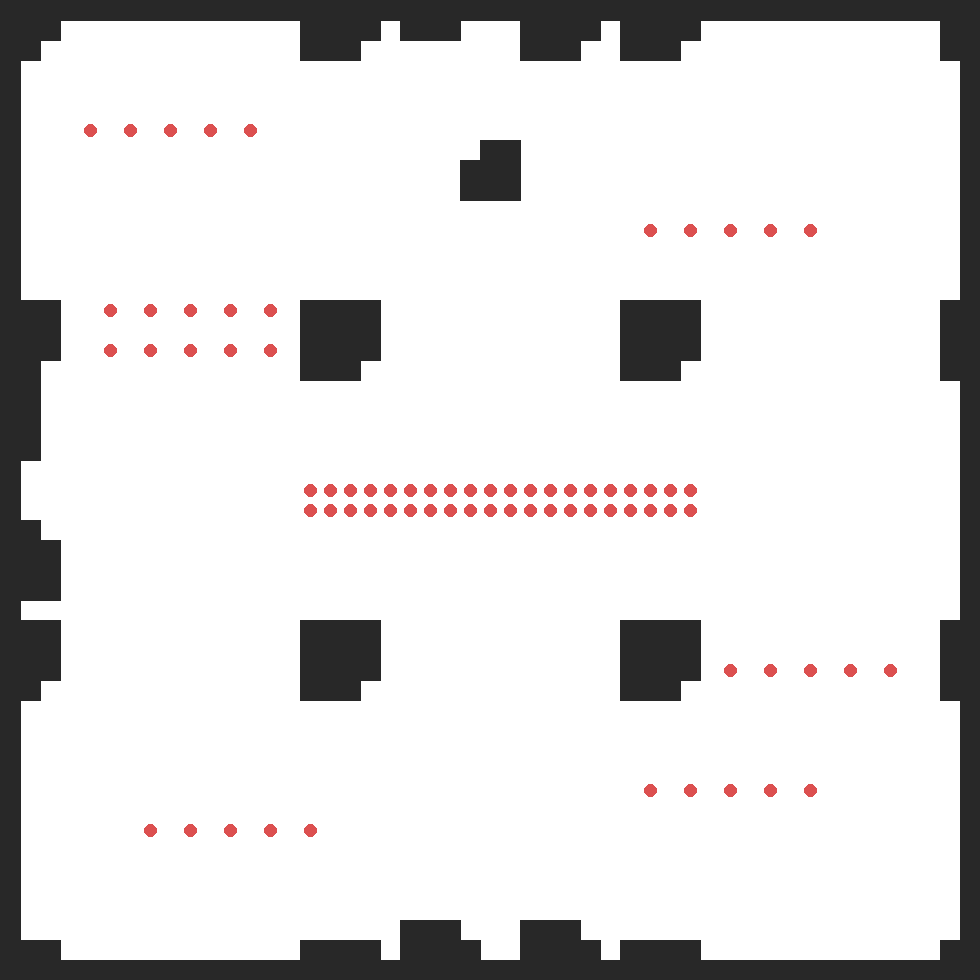
\includegraphics[width=0.55\textwidth]{map_arena.png}
        \caption{Модифицированная карта <<Arena>> размером $49 \times 49$ клеток, использованная при сравнении $A^*$ и $D^*$\,Lite.}
        \label{fig:map_arena}
    \end{figure}

    Параметр сложности конфигурации ($n$\_dst) определялся как минимальное манхэттенское расстояние
    между точками старта и финиша: $d_M = |x_{\text{start}} - x_{\text{goal}}| + |y_{\text{start}} - y_{\text{goal}}| \geq n$.
    Для каждой итерации (от 0\_dst до 70\_dst) генерировалось 1000 случайных пар точек,
    что обеспечило высокую статистическую достоверность.

    В ходе тестов от 1 до 15 препятствий за каждый ход совершали случайное перемещение
    на одну клетку (вверх, вниз, влево или вправо). Для алгоритма $A^*$ проверялись две стратегии
    пересчёта: в режиме \textit{step} путь пересчитывается один раз в конце хода после того,
    как все препятствия совершили движение; в режиме \textit{change} путь пересчитывается мгновенно
    после каждого единичного перемещения любого препятствия.


    \subsection{Результаты экспериментов}

    Объединённые результаты экспериментов представлены на рисунке~\ref{fig:global_comparison_combined}. По оси абсцисс отложено число подвижных препятствий за ход (значение 0 соответствует статической среде, $1$--$15$ -- различным уровням динамики); по оси ординат -- среднее время построения или обновления маршрута в миллисекундах. Значения усреднены по всем пяти конфигурациям минимальной дистанции между стартом и целью (0\_dst, 10\_dst, 30\_dst, 50\_dst, 70\_dst). Для алгоритма $A^*$ приведены два режима перепланирования: \textit{step} (одно перепланирование в конце хода) и \textit{change} (перепланирование после каждого единичного перемещения препятствия). Алгоритм $D^*$\,Lite показан одной кривой, поскольку в обоих режимах его поведение почти не различается.

    \begin{figure}[H]
        \centering
        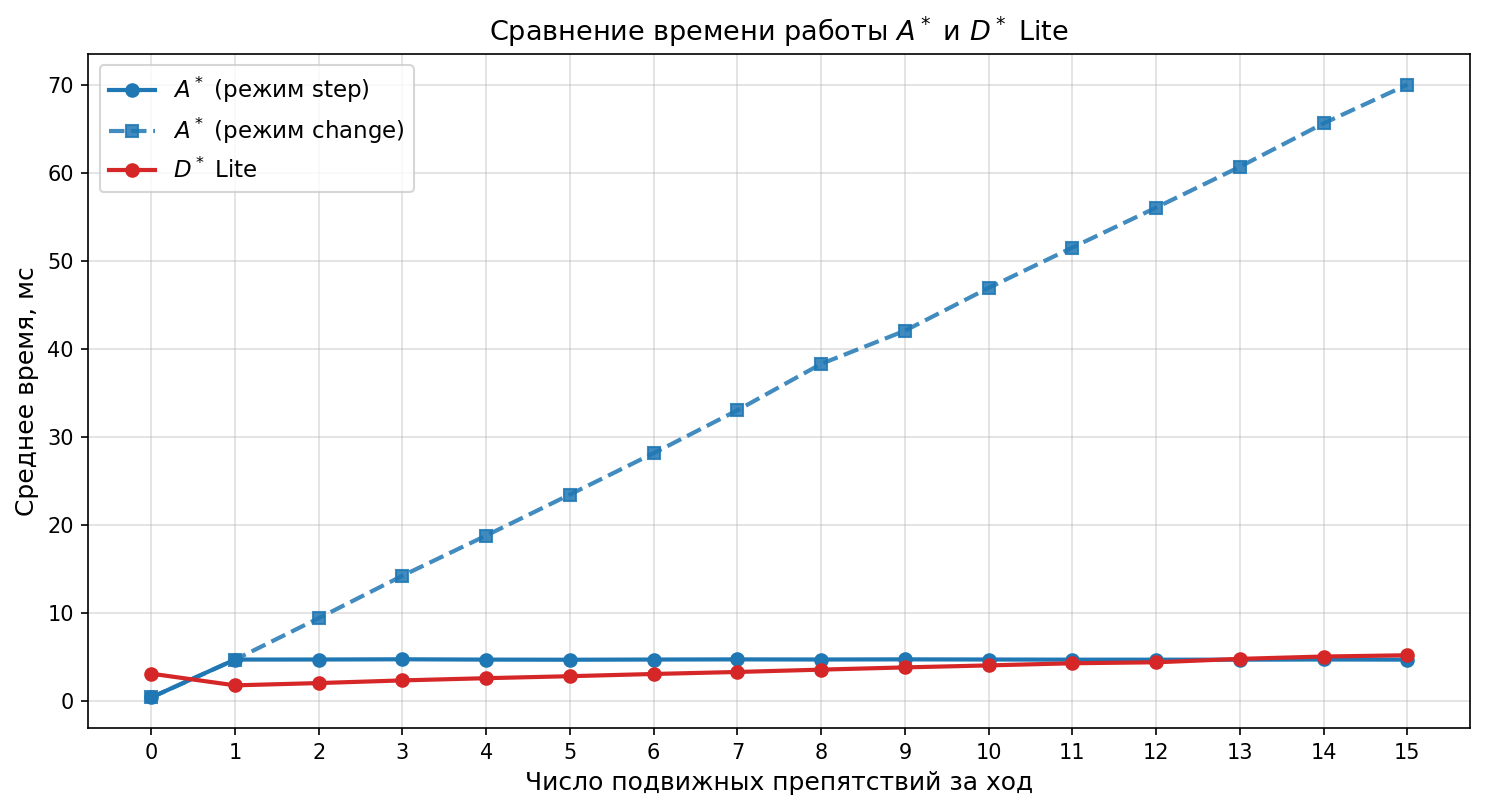
\includegraphics[width=0.95\textwidth]{global_comparison_combined.png}
        \caption{Сравнение времени работы $A^*$ и $D^*$\,Lite при различной интенсивности изменений карты (усреднение по всем дистанциям между стартом и целью).}
        \label{fig:global_comparison_combined}
    \end{figure}

    \subsection{Анализ производительности в статической среде}

    В условиях неизменной карты (значение 0 на оси абсцисс рис.~\ref{fig:global_comparison_combined}) алгоритм $A^*$ показал преимущество. Его вычислительная сложность при разовом поиске значительно ниже, чем у конкурента: среднее время поиска по всем дистанциям составляет около $0{,}5$ мс, что подтверждает оптимальность $A^*$ для однократного планирования на статичной карте.

    $D^*$\,Lite демонстрирует более тяжеловесный старт -- около $3$ мс в статике. Это связано с накладными расходами на инициализацию сложных структур данных и приоритетных очередей, которые необходимы алгоритму для будущей адаптации к изменениям, но в статике являются избыточными.

    \subsection{Анализ производительности в динамической среде}

    При введении движущихся препятствий ситуация кардинально меняется (правая часть рис.~\ref{fig:global_comparison_combined}). Ключевым фактором становится способность алгоритма переиспользовать предыдущие вычисления.

    Алгоритм $A^*$ не обладает <<памятью>> о предыдущих итерациях, что приводит к полной перепланировке при каждом изменении карты. В режиме \textit{change} среднее время пересчёта растёт линейно с числом изменений за ход: от $\approx 9$ мс при $1$ препятствии до $\approx 70$ мс при $15$ препятствиях, поскольку алгоритм выполняет $N$ полноценных поисков за один цикл. Режим \textit{step} снижает нагрузку до $\approx 4{,}5$ мс независимо от числа препятствий (одно перепланирование на ход) и оказывается сопоставимым с $D^*$\,Lite по времени при высокой плотности изменений.

    Однако применимость режима \textit{step} в реальных условиях ограничена: между моментами пересчёта робот следует устаревшему маршруту, полученному до перемещения препятствий, и не реагирует на промежуточные изменения карты. При высокой плотности динамики это означает, что часть хода робот движется по маршруту, который уже мог стать невалидным (например, проходит через клетку, занятую сместившимся препятствием), что повышает риск столкновения и приводит к небезопасным траекториям. В реализованной модели данная проблема исключена за счёт фиксированного порядка ходов: сначала перемещаются препятствия, затем робот пересчитывает маршрут и делает шаг -- всё в пределах одного такта моделирования. Режим \textit{change}, напротив, гарантирует реакцию на каждое изменение, но при $A^*$ обходится прямо пропорциональным ростом вычислительной стоимости. $D^*$\,Lite по существу обеспечивает поведение режима \textit{change} (реакцию на каждое изменение) ценой режима \textit{step} (постоянное время на ход), что и составляет его практическое преимущество.

    Алгоритм $D^*$\,Lite специально разработан для работы в меняющемся окружении. Его среднее время обработки изменений растёт очень умеренно -- от $\approx 1{,}7$ мс при $1$ препятствии до $\approx 5$ мс при $15$ препятствиях. На карте <<Arena>> это проявляется наиболее ярко: поскольку объекты перемещаются всего на одну клетку, $D^*$\,Lite обновляет лишь локальные веса в своём графе, не затрагивая те части пути, которые остались актуальными. Это делает его в $12$--$15$ раз быстрее $A^*$ в режиме \textit{change} при высокой плотности динамики.

    Наблюдаемые результаты подтверждают принципиальное различие вычислительных стратегий алгоритмов.
    В статической среде $A^*$ демонстрирует явное превосходство благодаря элегантной архитектуре
    поиска в графе. Однако в динамической среде при росте числа препятствий и частоте обновлений
    преимущество полностью переходит к $D^*$ Lite за счет инкрементального характера обновлений.
    Разрыв в производительности становится катастрофичным для $A^*$ в режиме \textit{change}:
    при 15 движущихся объектах производительность падает по крайней мере в 15...20 раз по сравнению с $D^*$ Lite.

    \subsection{Выводы по главе}

    Проведенное сравнение показало, что выбор алгоритма существенно зависит от характера среды и требований приложения.

    \begin{table}[H]
        \centering
        \footnotesize
        \caption{Сравнительные характеристики $A^*$ и $D^*$ Lite}
        \label{tab:comparison}
        \begin{tabular}{|>{\raggedright\arraybackslash}p{0.40\textwidth}|>{\centering\arraybackslash}p{0.26\textwidth}|>{\centering\arraybackslash}p{0.26\textwidth}|}
            \hline
            \textbf{Параметр сравнения} & \textbf{$A^*$ (A-Star)} & \textbf{$D^*$ Lite} \\
            \hline
            Статическая скорость (мин--макс, среднее) & 0{,}22--0{,}74 мс ($\sim$0{,}46 мс) & 1{,}26--5{,}69 мс ($\sim$3{,}16 мс) \\
            \hline
            Динамика: режим \textit{step} (мин--макс, среднее) & 1{,}98--10{,}70 мс ($\sim$4{,}76 мс) & 0{,}92--9{,}29 мс ($\sim$3{,}59 мс) \\
            \hline
            Динамика: режим \textit{change} (мин--макс, среднее) & 2{,}04--155{,}58 мс ($\sim$37{,}55 мс) & 0{,}92--9{,}33 мс ($\sim$3{,}59 мс) \\
            \hline
        \end{tabular}
    \end{table}

    Для разового построения пути в статических условиях классический $A^*$ эффективен благодаря 
    простоте и низким накладным расходам. Однако для задач с регулярными изменениями карты, 
    особенно при интенсивной динамике, значительно более устойчивым по времени выполнения 
    оказывается $D^*$ Lite.

    Таким образом, эксперимент подтверждает, что для задач разовой навигации предпочтителен $A^*$
    благодаря его вычислительной легкости. Однако в условиях интенсивной динамики и необходимости
    мгновенной реакции на изменения среды (режим \textit{change}) $D^*$ Lite является единственным
    масштабируемым решением, гарантирующим предсказуемое время отклика.

    \newpage

    \section{Алгоритмы локального планирования}

    В данной главе рассматриваются алгоритмы локального планирования, выбранные в обзоре для подробного исследования: базовый стохастический предсказательный контроллер MPPI и его риск-чувствительное расширение RA-MPPI, а также их модификации с явным прогнозом подвижных препятствий (далее MPPI-pred и RA-MPPI-pred). Сначала описаны формальные модели обоих алгоритмов и их пошаговые схемы, затем приводится экспериментальное сравнение в статической и динамической средах.

    \subsection{Общие концепции алгоритмов MPPI и RA-MPPI}

    Оба рассматриваемых алгоритма относятся к семейству стохастических предсказательных контроллеров. На каждом шаге оптимизация ведётся не аналитически, а по выборке возмущённых траекторий; решение получается как взвешенная комбинация сэмплов, где более качественные траектории получают больший вес.

    \paragraph{Алгоритм MPPI.}

    \textbf{MPPI (Model Predictive Path Integral)} --- стохастический локальный планировщик,
    основанный на одновременной оценке большого числа возможных траекторий~\cite{mppis, mppi}.
    На каждом шаге алгоритм оценивает $K$ \emph{возмущённых траекторий} --
    пробных траекторий, разыгрываемых вперёд по модели динамики робота из его текущей позиции:
    на каждом шаге горизонта $t = 1, \dots, T$ к \emph{номинальному управлению} $\bar{u}_t$ --
    базовой последовательности управляющих воздействий, относительно которой ведётся сэмплирование (в данной реализации это единичный вектор, направленный к цели; в общем случае MPPI использует управляющую последовательность, оптимизированную на предыдущем такте) --
    добавляется гауссовский шум $\varepsilon_t^{(k)} \sim \mathcal{N}(0,\sigma^2 I)$,
    после чего получившееся управление $\bar{u}_t + \varepsilon_t^{(k)}$ подаётся в модель динамики и определяет следующее состояние робота.
    Каждая такая траектория оценивается скалярной функцией стоимости
    $$
    J_k \;=\; \sum_{t=1}^{T} \Big[\, c_{\text{obst}} \cdot \mathrm{I}\!\left[\, s_t^{(k)} \in \mathcal{O}\, \right]
          + w_s \cdot d(s_t^{(k)}, g)\, \Big]
          \;+\; w_T \cdot d(s_T^{(k)}, g),
    $$
    где $s_t^{(k)}$ --- состояние $k$-й траектории на шаге $t$,
    $\mathcal{O}$ --- множество клеток-препятствий,
    $\mathrm{I}[\,\cdot\,]$ --- индикатор (равен $1$, если условие выполнено, и $0$ иначе),
    $d(s,g)$ --- евклидово расстояние от состояния $s$ до цели $g$,
    $w_s$ и $w_T$ --- весовые коэффициенты промежуточного и терминального слагаемых,
    $c_{\text{obst}}$ --- штраф за столкновение с препятствием.
    Терминальное слагаемое $w_T \cdot d(s_T^{(k)}, g)$ суммируется поверх
    последнего слагаемого ряда и тем самым усиливает значимость финальной точки траектории.

    После того как все траектории оценены, управление обновляется как взвешенная сумма возмущений, где каждая траектория получает \emph{вес Больцмана} -- экспоненциально убывающий по стоимости и нормированный так, чтобы веса в сумме давали единицу:
    $$
    w_k \;=\; \frac{\exp\!\left(-\dfrac{J_k - J_{\min}}{\lambda}\right)}
                   {\displaystyle\sum_{j=1}^{K} \exp\!\left(-\dfrac{J_j - J_{\min}}{\lambda}\right)},
    \qquad \sum_{k=1}^{K} w_k = 1.
    $$
    Чем меньше стоимость траектории, тем больший вклад она вносит в итоговое управление. Параметр $\lambda > 0$ задаёт «температуру» распределения: при малых $\lambda$ управление определяется преимущественно одной траекторией с минимальной стоимостью (эквивалент жёсткого $\arg\min_k J_k$), при больших -- равномерно усредняется по всему ансамблю. Вычитание $J_{\min} = \min_j J_j$ из аргумента экспоненты не меняет значений нормированных весов, но предотвращает переполнение при больших стоимостях.

    Пошаговая схема работы алгоритма на каждом такте управления:
    \begin{enumerate}
        \item Зафиксировать номинальное управление $\bar{u}$ (направление к цели или ранее выбранное управление).
        \item Сгенерировать $K$ возмущённых траекторий: для каждой $k = 1, \dots, K$
            \begin{enumerate}
                \item на каждом шаге горизонта $t = 1, \dots, T$ взять гауссовское возмущение $\varepsilon_t^{(k)} \sim \mathcal{N}(0, \sigma^2 I)$;
                \item развернуть траекторию $s_0^{(k)}, s_1^{(k)}, \dots, s_T^{(k)}$, применяя управление $\bar{u}_t + \varepsilon_t^{(k)}$ через модель динамики;
                \item вычислить стоимость $J_k$ по формуле выше.
            \end{enumerate}
        \item Найти $J_{\min} = \min_j J_j$ и вычислить веса Больцмана $w_k$ по формуле выше.
        \item Сформировать обновлённое управление как взвешенную сумму возмущений: $u_t^\star = \bar{u}_t + \sum_{k=1}^{K} w_k \, \varepsilon_t^{(k)}$.
        \item Применить $u_1^\star$ к роботу, сдвинуть управляющую последовательность и перейти к следующему такту.
    \end{enumerate}

    \paragraph{Алгоритм RA-MPPI.}

    \textbf{RA-MPPI (Risk-Aware MPPI)} расширяет MPPI явным учётом \emph{хвостового риска} -- ожидаемых потерь в редких, но неблагоприятных сценариях исполнения управления, когда даже хорошая в среднем траектория может реализоваться существенно хуже из-за случайных отклонений~\cite{ra_mppi}. Базовый MPPI рассматривает только одну стоимость на траекторию и не различает траектории с одинаковым средним, но разной устойчивостью к таким отклонениям; RA-MPPI устраняет этот недостаток, дополнительно оценивая, насколько плохо траектория ведёт себя в худших возможных реализациях.

    Для количественной оценки используется мера \emph{CVaR (Conditional Value-at-Risk, условная стоимость под риском)} -- среднее значение стоимости среди заданного процента самых неблагоприятных сэмплированных реализаций. Если параметр $\alpha \in [0, 1]$ задаёт уровень доверия, то CVaR$_\alpha$ вычисляется как среднее по худшим $(1-\alpha) \cdot 100\%$ значениям стоимости: например, при $\alpha = 0{,}8$ это среднее по $20\%$ самых худших сэмплов.

    Для каждой из $K$ номинальных траекторий разыгрывается $N_d$ возмущённых \emph{роллаутов} -- дополнительных симуляций траектории на горизонте прогноза, в которых к управлению добавляется случайный шум $\boldsymbol{\delta} \sim \mathcal{N}(0, \sigma_d^2 I)$, имитирующий неопределённость исполнения управления (по своей сути роллаут -- это просто прогон управляющей последовательности через модель динамики, аналогично сэмплированию траекторий в MPPI).
    По полученным $N_d$ стоимостям вычисляется CVaR$_\alpha$ --- среднее по худшим
    $\lceil (1-\alpha) N_d \rceil$ значениям:
    $$
    \widehat{J}_k = J_k + \gamma \cdot
    \operatorname{CVaR}_{\alpha}\!\bigl(\{J_k^{(n)}\}_{n=1}^{N_d}\bigr),
    $$
    где $J_k$ --- стоимость номинального роллаута, $J_k^{(n)}$ --- стоимость $n$-го возмущённого роллаута,
    $\gamma > 0$ --- вес штрафа за риск.
    Штраф добавляется только тогда, когда CVaR превышает заданный порог $C_u$;
    иначе $\widehat{J}_k = J_k$.
    Затем стандартная схема взвешивания Больцмана применяется к скорректированным стоимостям $\widehat{J}_k$,
    и RA-MPPI сводится к классическому MPPI, если CVaR ни для одной траектории не нарушает порог.

    Пошаговая схема работы алгоритма:
    \begin{enumerate}
        \item Для каждой из $K$ номинальных траекторий выполнить шаги 2(a)--2(c) MPPI: получить $J_k$ и сохранить последовательность возмущений $\varepsilon^{(k)}$.
        \item Для каждой номинальной траектории $k$ оценить хвостовой риск:
            \begin{enumerate}
                \item разыграть $N_d$ дополнительных возмущённых роллаутов, добавляя к управлению шум $\boldsymbol{\delta}_t^{(n)} \sim \mathcal{N}(0, \sigma_d^2 I)$;
                \item вычислить стоимости $J_k^{(1)}, \dots, J_k^{(N_d)}$;
                \item отсортировать стоимости и взять среднее по худшим $\lceil (1-\alpha) N_d \rceil$ значениям -- это CVaR$_\alpha$.
            \end{enumerate}
        \item Скорректировать стоимость номинальной траектории: если CVaR$_\alpha$ превышает порог $C_u$, то $\widehat{J}_k = J_k + \gamma \cdot \mathrm{CVaR}_\alpha$, иначе $\widehat{J}_k = J_k$.
        \item Применить взвешивание Больцмана к скорректированным стоимостям $\widehat{J}_k$ и сформировать обновлённое управление как у MPPI.
    \end{enumerate}

    Ключевое отличие RA-MPPI от MPPI -- дополнительный внутренний цикл по $N_d$ роллаутам для каждой из $K$ номинальных траекторий, что увеличивает вычислительную стоимость в $N_d$ раз. Взамен траектории, по которым существует существенный риск столкновения при возмущениях исполнения, получают повышенный штраф и меньший вес в итоговом управлении.

    \subsection{Учёт прогноза подвижных препятствий}

    Базовые версии MPPI и RA-MPPI на каждом шаге работают с одномоментным срезом среды:
    функция стоимости $J_k$ начисляет штраф только за столкновение с клетками, занятыми
    в текущий момент времени. Это означает, что роллауты на горизонте $T$ оценивают траектории
    относительно неизменной карты, даже если на следующем такте часть препятствий сместится.
    В разреженной динамике такая модель приближает реальность с систематической ошибкой:
    робот может выбрать траекторию, проходящую через клетку, которую препятствие займёт через
    несколько шагов.

    Для коррекции этого эффекта предложены варианты MPPI-pred и RA-MPPI-pred,
    которые на каждом шаге дополнительно получают список наблюдённых перемещений
    препятствий за прошедший такт $\mathcal{D} = \{(x_i, y_i, v_{x,i}, v_{y,i})\}$,
    где $(x_i, y_i)$ --- текущая позиция $i$-го объекта, $(v_{x,i}, v_{y,i})$ --- его
    одношаговая скорость, вычисленная как разность последних двух наблюдаемых клеток.
    Внутри роллаута для каждого шага $t \in \{1, \dots, T\}$ предсказанная позиция
    объекта берётся как линейная экстраполяция $(\hat{x}_i^{(t)}, \hat{y}_i^{(t)}) =
    (x_i + t v_{x,i}, y_i + t v_{y,i})$, а к стоимости траектории добавляется
    мягкий штраф, активирующийся в окрестности предсказанной точки:
    $$
    \Delta J^{(\text{pred})}_k \;=\; \sum_{t=1}^{T} \sum_{i \in \mathcal{D}}
    \frac{w_p \cdot c_{\text{obst}}}{1 + \rho_i^{(t)}} \cdot
    \mathrm{I}\!\left[\rho_i^{(t)} \le 1\right],
    \qquad
    \rho_i^{(t)} = \bigl|x^{(k)}_t - \hat{x}_i^{(t)}\bigr| +
                   \bigl|y^{(k)}_t - \hat{y}_i^{(t)}\bigr|,
    $$
    где $\rho_i^{(t)}$ --- манхэттенское расстояние от $k$-й роллаут-траектории до
    предсказанной позиции $i$-го объекта на шаге $t$, а $w_p \in [0, 1]$ --- весовой
    коэффициент прогнозного слагаемого. В RA-MPPI-pred прогнозный штраф применяется как
    к номинальному роллауту, так и к возмущённым роллаутам внутри CVaR-оценки,
    поэтому риск столкновения с предсказанной траекторией препятствия попадает
    в хвостовое распределение наравне со стохастической неопределённостью управления.
    Полная функция стоимости в обоих расширениях имеет вид
    $J^{(\text{pred})}_k = J_k + \Delta J^{(\text{pred})}_k$
    для MPPI-pred и
    $\widehat{J}^{(\text{pred})}_k = J^{(\text{pred})}_k + \gamma \cdot \operatorname{CVaR}_{\alpha}(\{J_k^{(n)} + \Delta J^{(\text{pred}, n)}_k\})$
    для RA-MPPI-pred.

    Принципиально модель прогноза остаётся максимально консервативной:
    она использует только один последний наблюдаемый шаг для оценки скорости,
    не использует поведенческой модели среды и не накладывает дополнительных ограничений
    на параметры базовых планировщиков. Это позволяет рассматривать MPPI-pred и RA-MPPI-pred
    как минимальное расширение, проверяющее ценность даже грубого линейного прогноза
    в задаче навигации со случайно блуждающими препятствиями.

    \subsection{Модель и условия эксперимента}

    Эксперименты выполнялись на том же бенчмарке <<Arena>>, что и сравнение глобальных планировщиков: карта размером $49 \times 49$ клеток со статическими препятствиями и группами динамических объектов.

    Реализованная программная модель является \emph{гибридной}: карта и итоговое перемещение робота за один такт дискретны, а само сэмплирование MPPI/RA-MPPI выполняется в континуальном пространстве скоростей -- то есть скорость робота при роллауте представлена двумерным вектором с вещественными компонентами $(v_x, v_y) \in \mathbb{R}^2$ и может принимать любые значения из непрерывного диапазона, а не выбирается из небольшого фиксированного набора направлений (как, например, в восьмисвязной сетке). Конкретно:
    \begin{itemize}
        \item \emph{Карта} представлена сеточной структурой $49 \times 49$ клеток, на которой расположены статические и подвижные препятствия.
        \item \emph{Состояние при роллауте} -- континуальное: положение робота в процессе симуляции хранится в виде вещественных координат $(x, y)$, что позволяет применять стандартный аппарат MPPI с непрерывной динамикой.
        \item \emph{Номинальное управление} $\bar{u}$ -- двумерный вектор скорости, направленный от текущей клетки к цели и нормированный на единичную длину.
        \item \emph{Возмущения} $\varepsilon_t^{(k)} \sim \mathcal{N}(0, \sigma^2 I)$ -- континуальные двумерные гауссовские шумы, генерируемые из равномерных случайных чисел \emph{преобразованием Бокса--Мюллера} -- стандартным приёмом, который из пары независимых равномерных значений $u_1, u_2 \in (0, 1]$ строит пару независимых нормально распределённых значений по формулам $z_1 = \sqrt{-2\ln u_1}\cos(2\pi u_2)$ и $z_2 = \sqrt{-2\ln u_1}\sin(2\pi u_2)$. На каждом шаге горизонта возмущения добавляются к номинальному управлению, после чего получившаяся скорость подаётся в простейшую модель динамики $(x, y) \to (x + v_x, y + v_y)$.
        \item \emph{Проверка препятствий} при роллауте дискретна: континуальные координаты на каждом шаге горизонта округляются до ближайшей клетки и сверяются со списком занятых; столкновение добавляет в стоимость траектории штраф $c_\text{obst}$.
        \item \emph{Применение итогового управления} тоже дискретно: после вычисления взвешенной суммы сэмплов результирующий вектор $u^\star$ проецируется на сетку, и робот за такт переходит в одну из соседних клеток, в направлении которой $u^\star$ указывает наиболее сильно.
    \end{itemize}
    Такая схема позволяет использовать стандартный MPPI (с непрерывными управлениями и гауссовскими возмущениями), сохранив дискретную сеточную модель карты и единообразную дискретизацию хода робота, характерную для бенчмарков по поиску пути.

    В данных экспериментах глобальные планировщики ($A^*$/$D^*$\,Lite) не использовались. В отличие от практической интеграции в навигационный стек Nav2 (см. главу 5), где локальный планировщик получает опорный маршрут от глобального, здесь локальные алгоритмы MPPI/RA-MPPI работают напрямую с координатами цели: номинальное управление задаётся как единичный вектор от текущей позиции к цели, без участия глобального плана. Это позволяет сравнивать локальные алгоритмы между собой в чистом виде, не смешивая их поведение с особенностями того или иного глобального планировщика.

    Все четыре планировщика использовали $K = 500$ сэмплов при горизонте $T = 12$ шагов,
    температурный параметр $\lambda = 1{,}5$, стандартное отклонение шума $\sigma = 0{,}8$,
    штраф за столкновение $c_{\text{obst}} = 200$, $w_s = 0{,}1$, $w_T = 15{,}0$.
    Для RA-MPPI и RA-MPPI-pred дополнительно задавались уровень доверия CVaR $\alpha = 0{,}8$,
    число возмущённых роллаутов $N_d = 20$, стандартное отклонение возмущений $\sigma_d = 0{,}5$,
    вес штрафа за риск $\gamma = 1{,}0$ и порог активации штрафа $C_u = 0$.
    Для MPPI-pred и RA-MPPI-pred вес прогнозного слагаемого был выставлен в $w_p = 0{,}5$,
    что соответствует половинному вкладу штрафа за прогнозируемое столкновение по сравнению с прямым.
    В качестве списка $\mathcal{D}$ на каждом шаге использовались координаты препятствий,
    переместившихся на предыдущем такте моделирования; неподвижные за этот такт объекты в прогноз
    не включались, поскольку их одношаговая скорость не определена.

    Из полного набора задач отбирались 100 случайных пар <<старт --- цель>>;
    ограничение на число шагов составляло 500 в статическом и 50\,000 в динамическом режиме.
    В отличие от тестов глобальных планировщиков, количество задач было ограничено 100
    ввиду большей вычислительной стоимости сэмплирующих алгоритмов на каждом шаге навигации.
    Аналогично предыдущим тестам, препятствия за каждый ход совершали случайное перемещение
    на одну клетку; тестировались три уровня загрузки: 1, 5 и 10 подвижных препятствий.

    В отличие от глобальных планировщиков, для которых основным критерием являлось время перепланирования,
    оценка локальных методов строилась на четырёх показателях: \textit{успешность} --- доля задач,
    для которых найден путь до цели; \textit{время планирования} (мс) --- суммарное реальное время выполнения
    построения пути; \textit{извилистость} --- отношение длины пути к прямому расстоянию до цели
    (1{,}0 соответствует прямолинейному маршруту); \textit{доля опасных сближений} ---
    доля шагов, на которых хотя бы одна из соседних по горизонтали или вертикали клеток являлась препятствием.

    \subsection{Результаты экспериментов}

    Измерения для статического режима представлены на рисунке~\ref{fig:local_static_comparison}.
    На графике сопоставляются успешность, число шагов, стабильность, извилистость,
    время планирования и доля опасных ситуаций для всех четырёх рассматриваемых
    планировщиков по 100 тестовым задачам.

    Измерения для динамического режима представлены на рисунке~\ref{fig:local_dynamic_comparison}.
    График отражает зависимость тех же шести показателей от числа подвижных препятствий
    (1, 5 или 10 объектов, перемещающихся за ход).

    \begin{figure}[H]
        \centering
        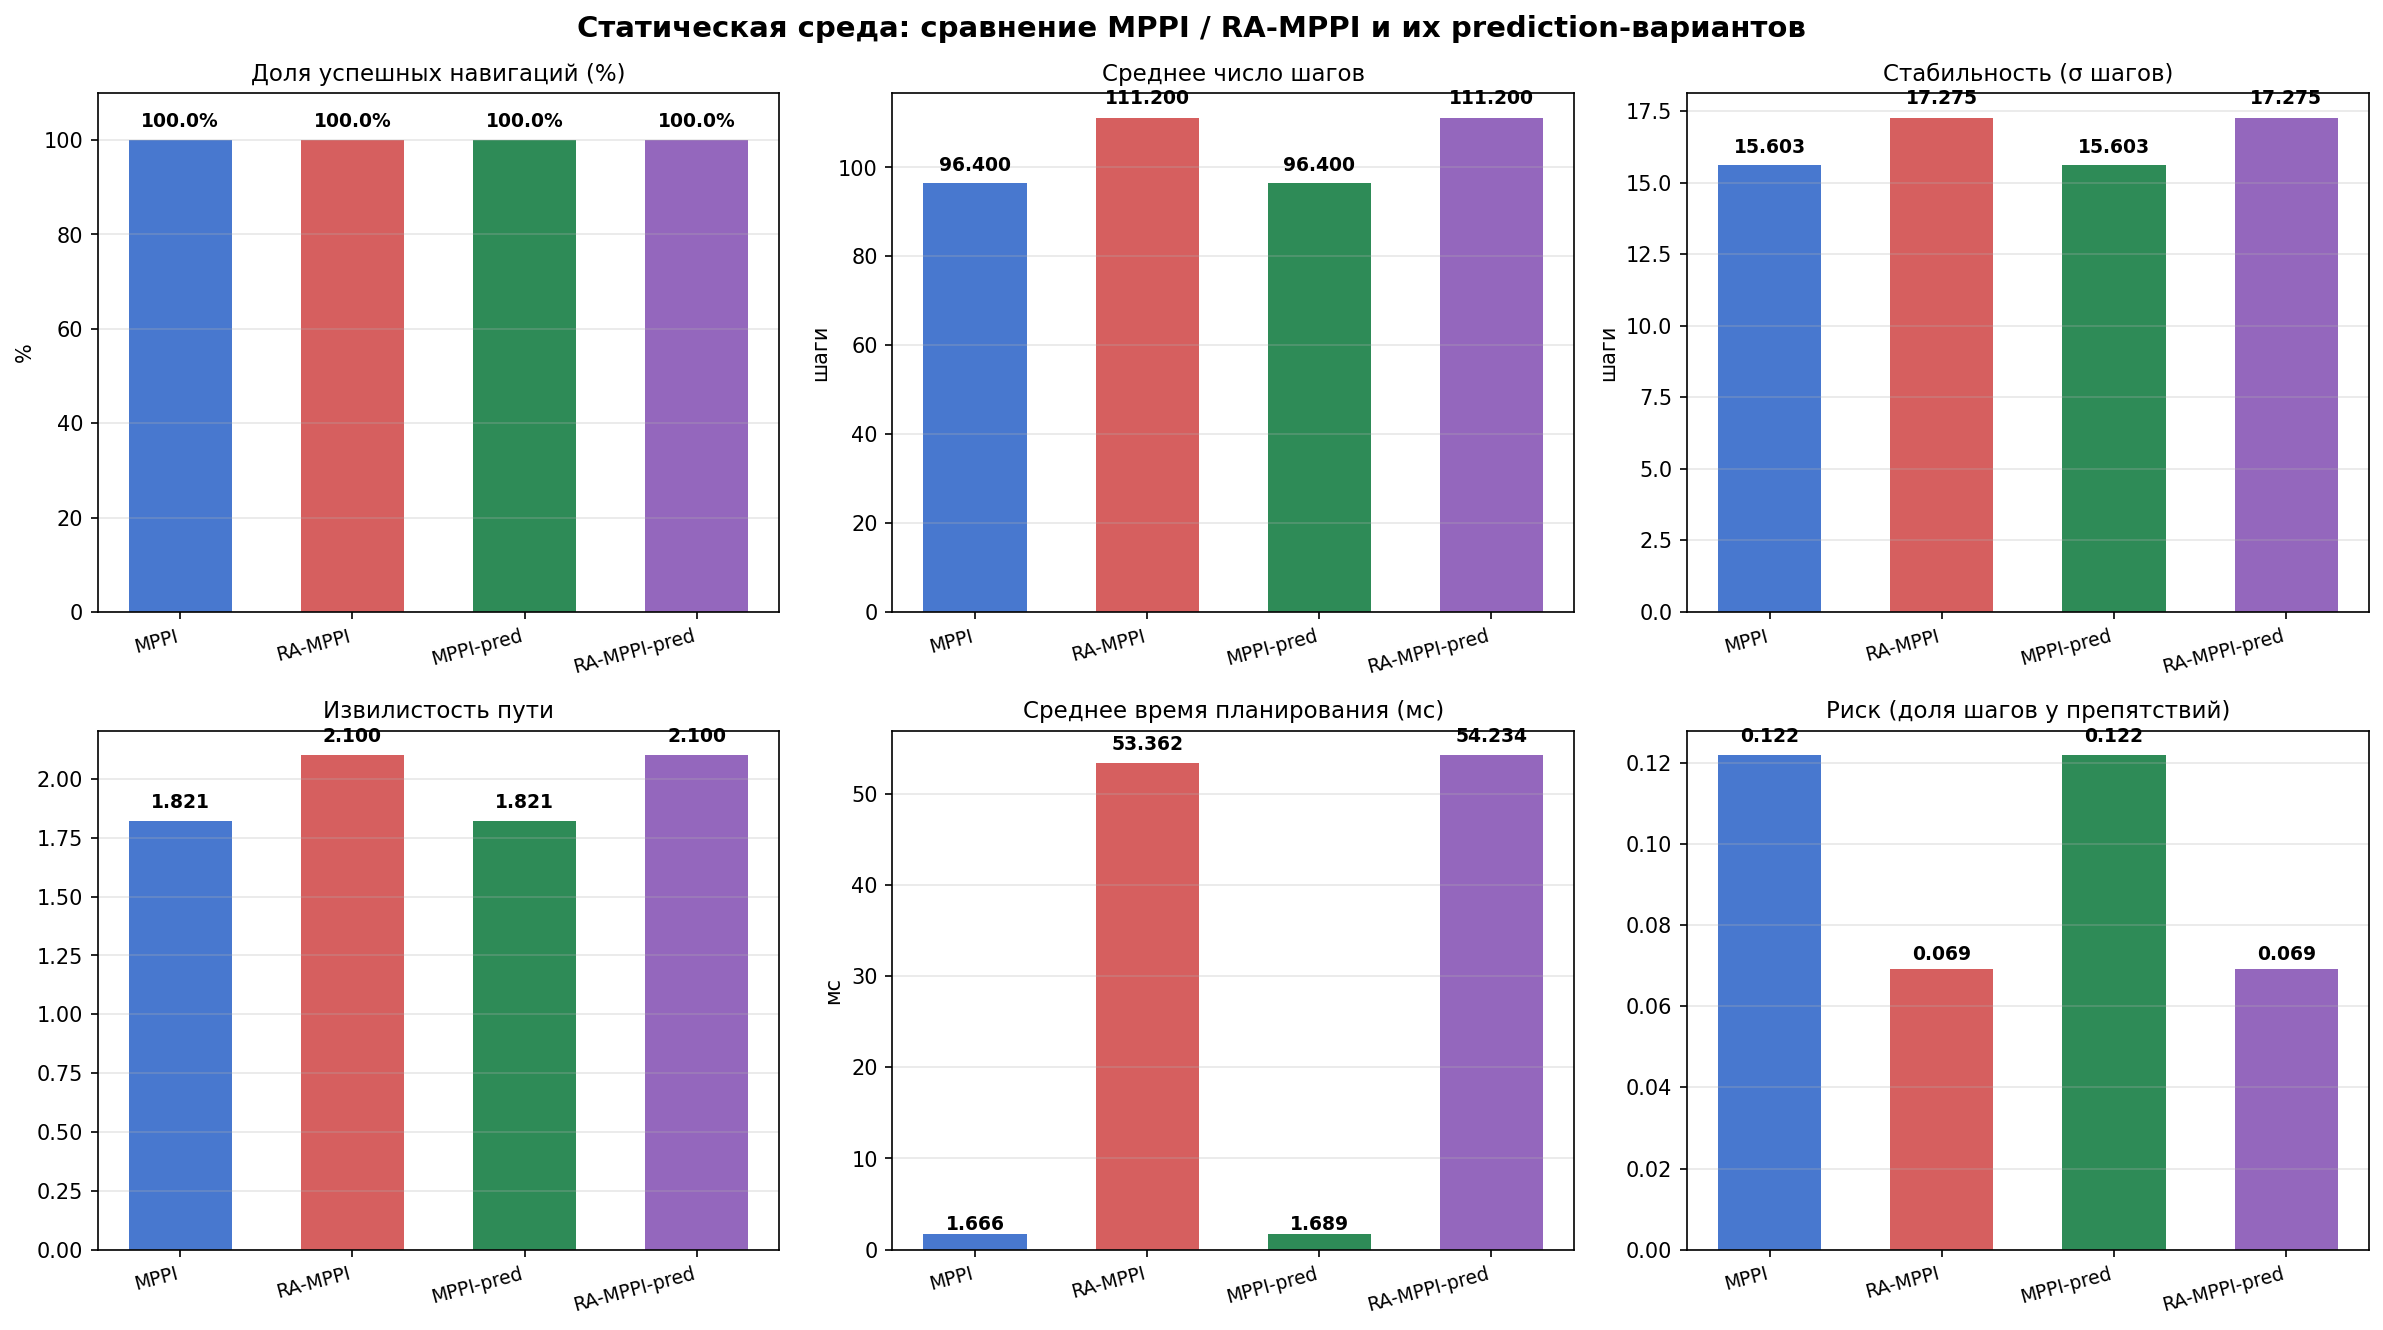
\includegraphics[width=0.95\textwidth]{local_static_comparison.png}
        \caption{Сравнение показателей MPPI, RA-MPPI и их prediction-вариантов в статической среде.}
        \label{fig:local_static_comparison}
    \end{figure}

    \begin{figure}[H]
        \centering
        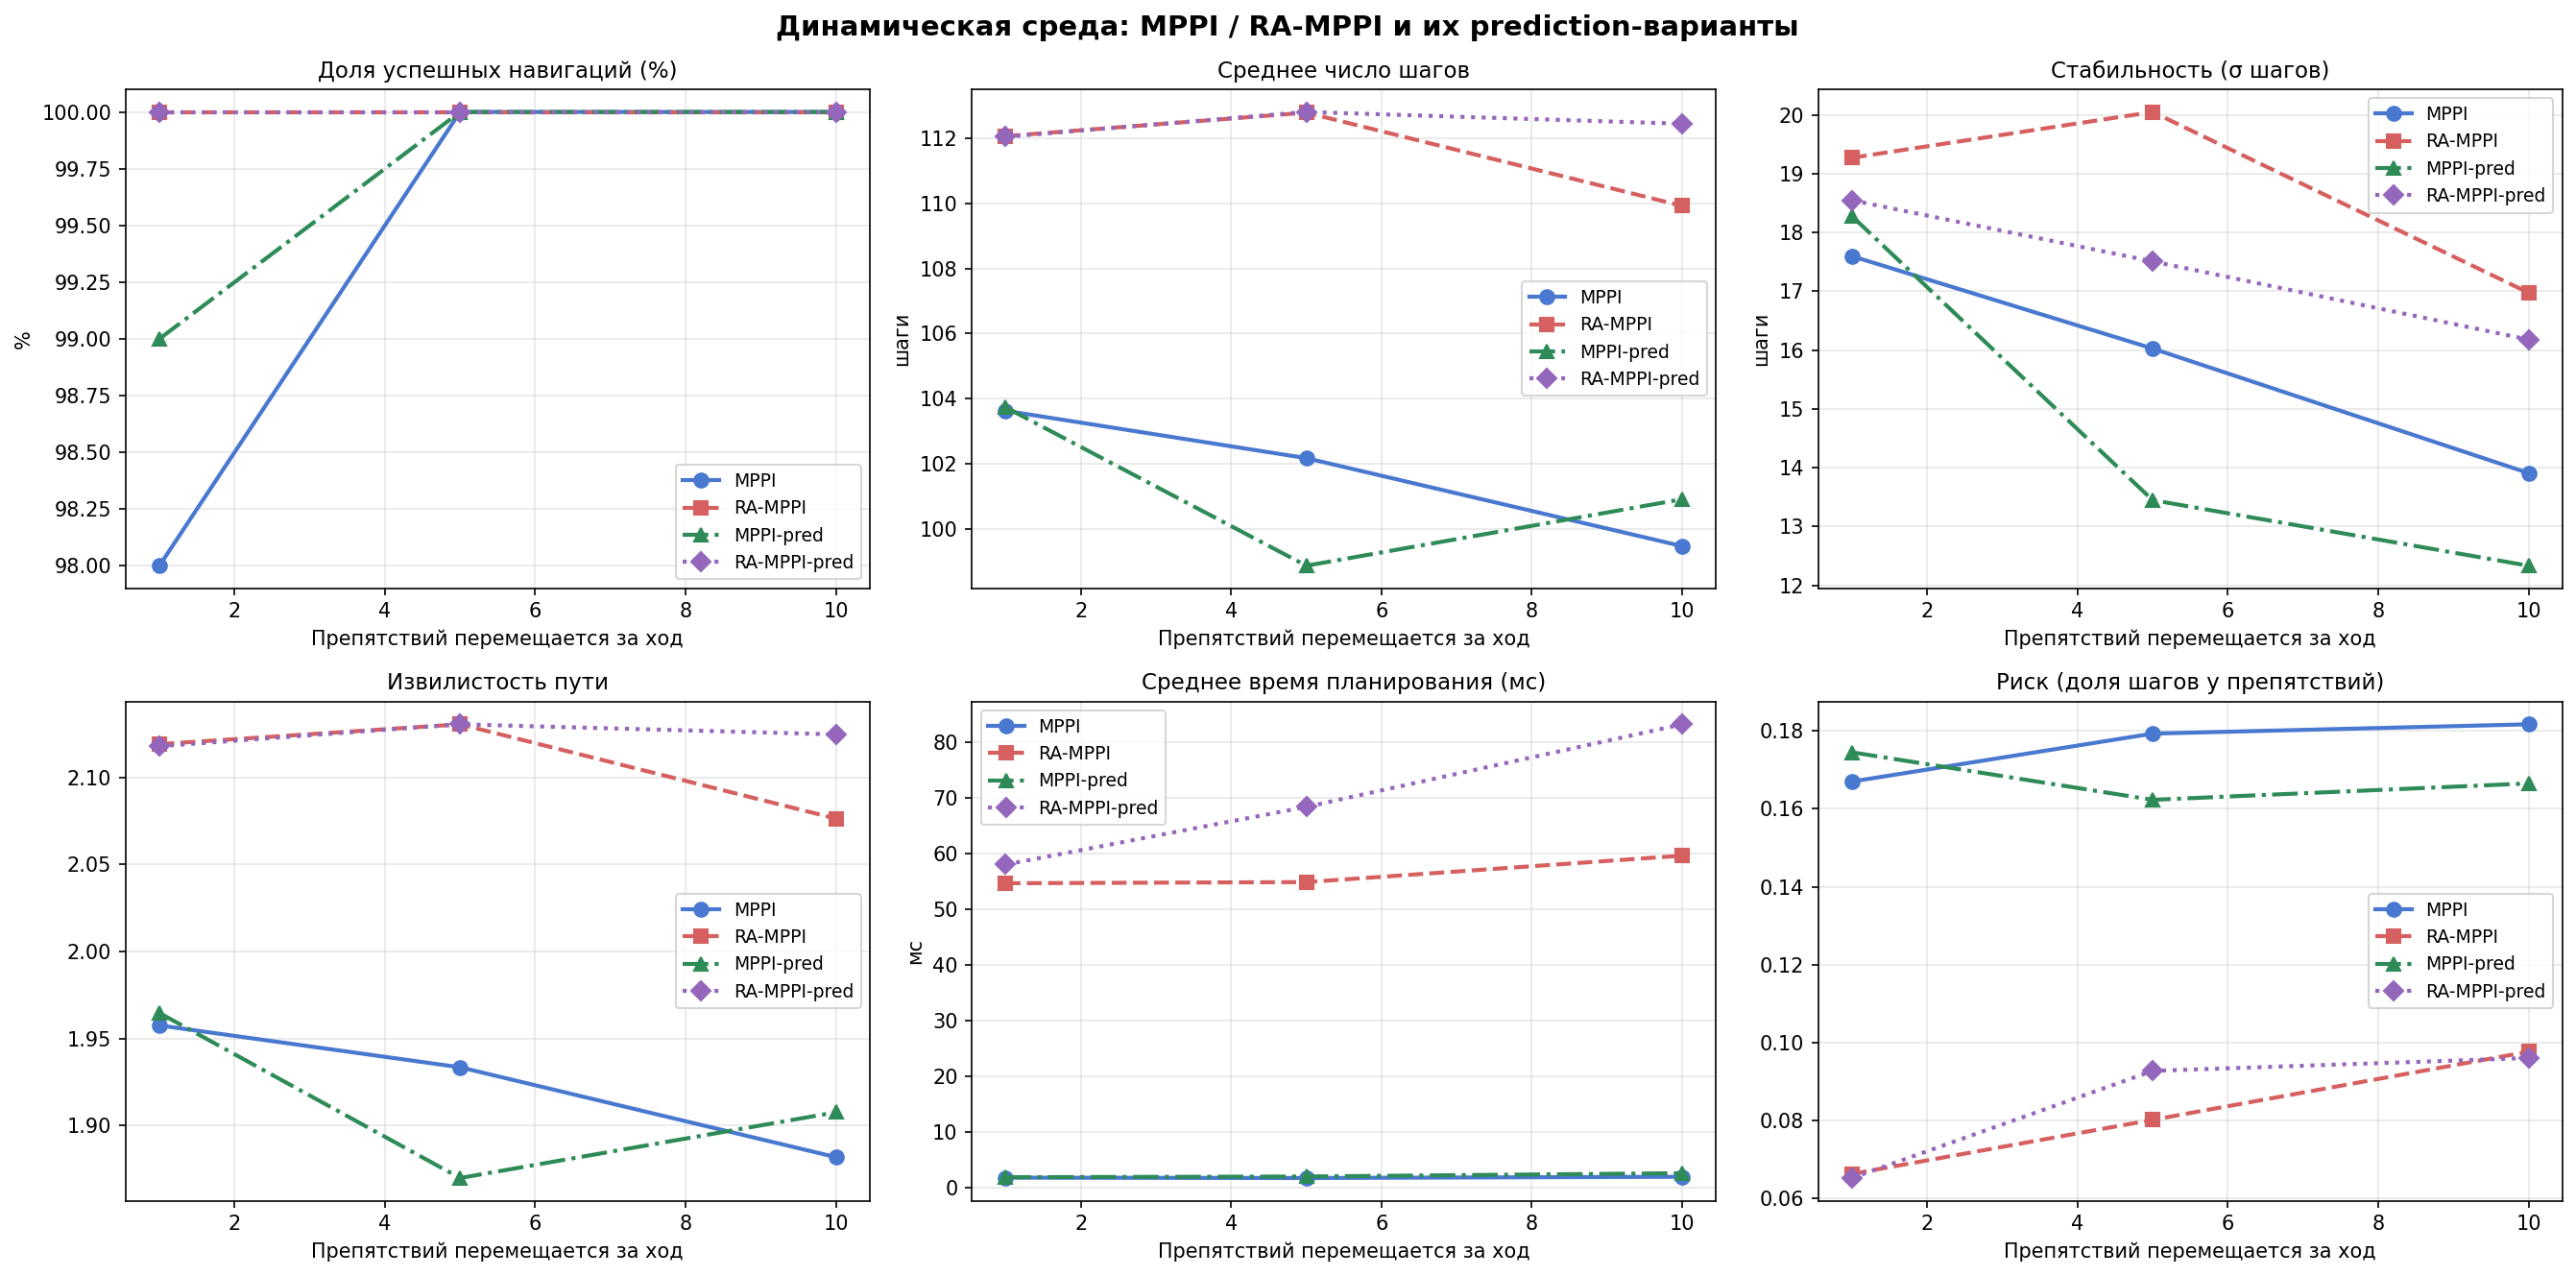
\includegraphics[width=0.95\textwidth]{local_dynamic_comparison.png}
        \caption{Сравнение показателей MPPI, RA-MPPI и их prediction-вариантов в динамической среде при различном числе подвижных препятствий.}
        \label{fig:local_dynamic_comparison}
    \end{figure}

    Для качественной иллюстрации различий между алгоритмами на рис.~\ref{fig:trace_local_planners} приведены траектории робота на одном и том же тестовом случае при средней плотности динамики (5 подвижных препятствий за ход). На карте показаны статические препятствия (серые блоки), следы подвижных препятствий (красные точки с угасающей прозрачностью по времени), стартовая позиция (зелёный круг) и цель (оранжевая звезда). MPPI и RA-MPPI находят похожие по геометрии маршруты длиной около $50$ шагов, тогда как RA-MPPI-pred в данном конкретном прогоне выбирает существенно более осторожный обход и тратит $88$ шагов: дополнительный штраф за предсказанные позиции подвижных объектов уводит траекторию в обход всей центральной зоны с препятствиями.

    \begin{figure}[H]
        \centering
        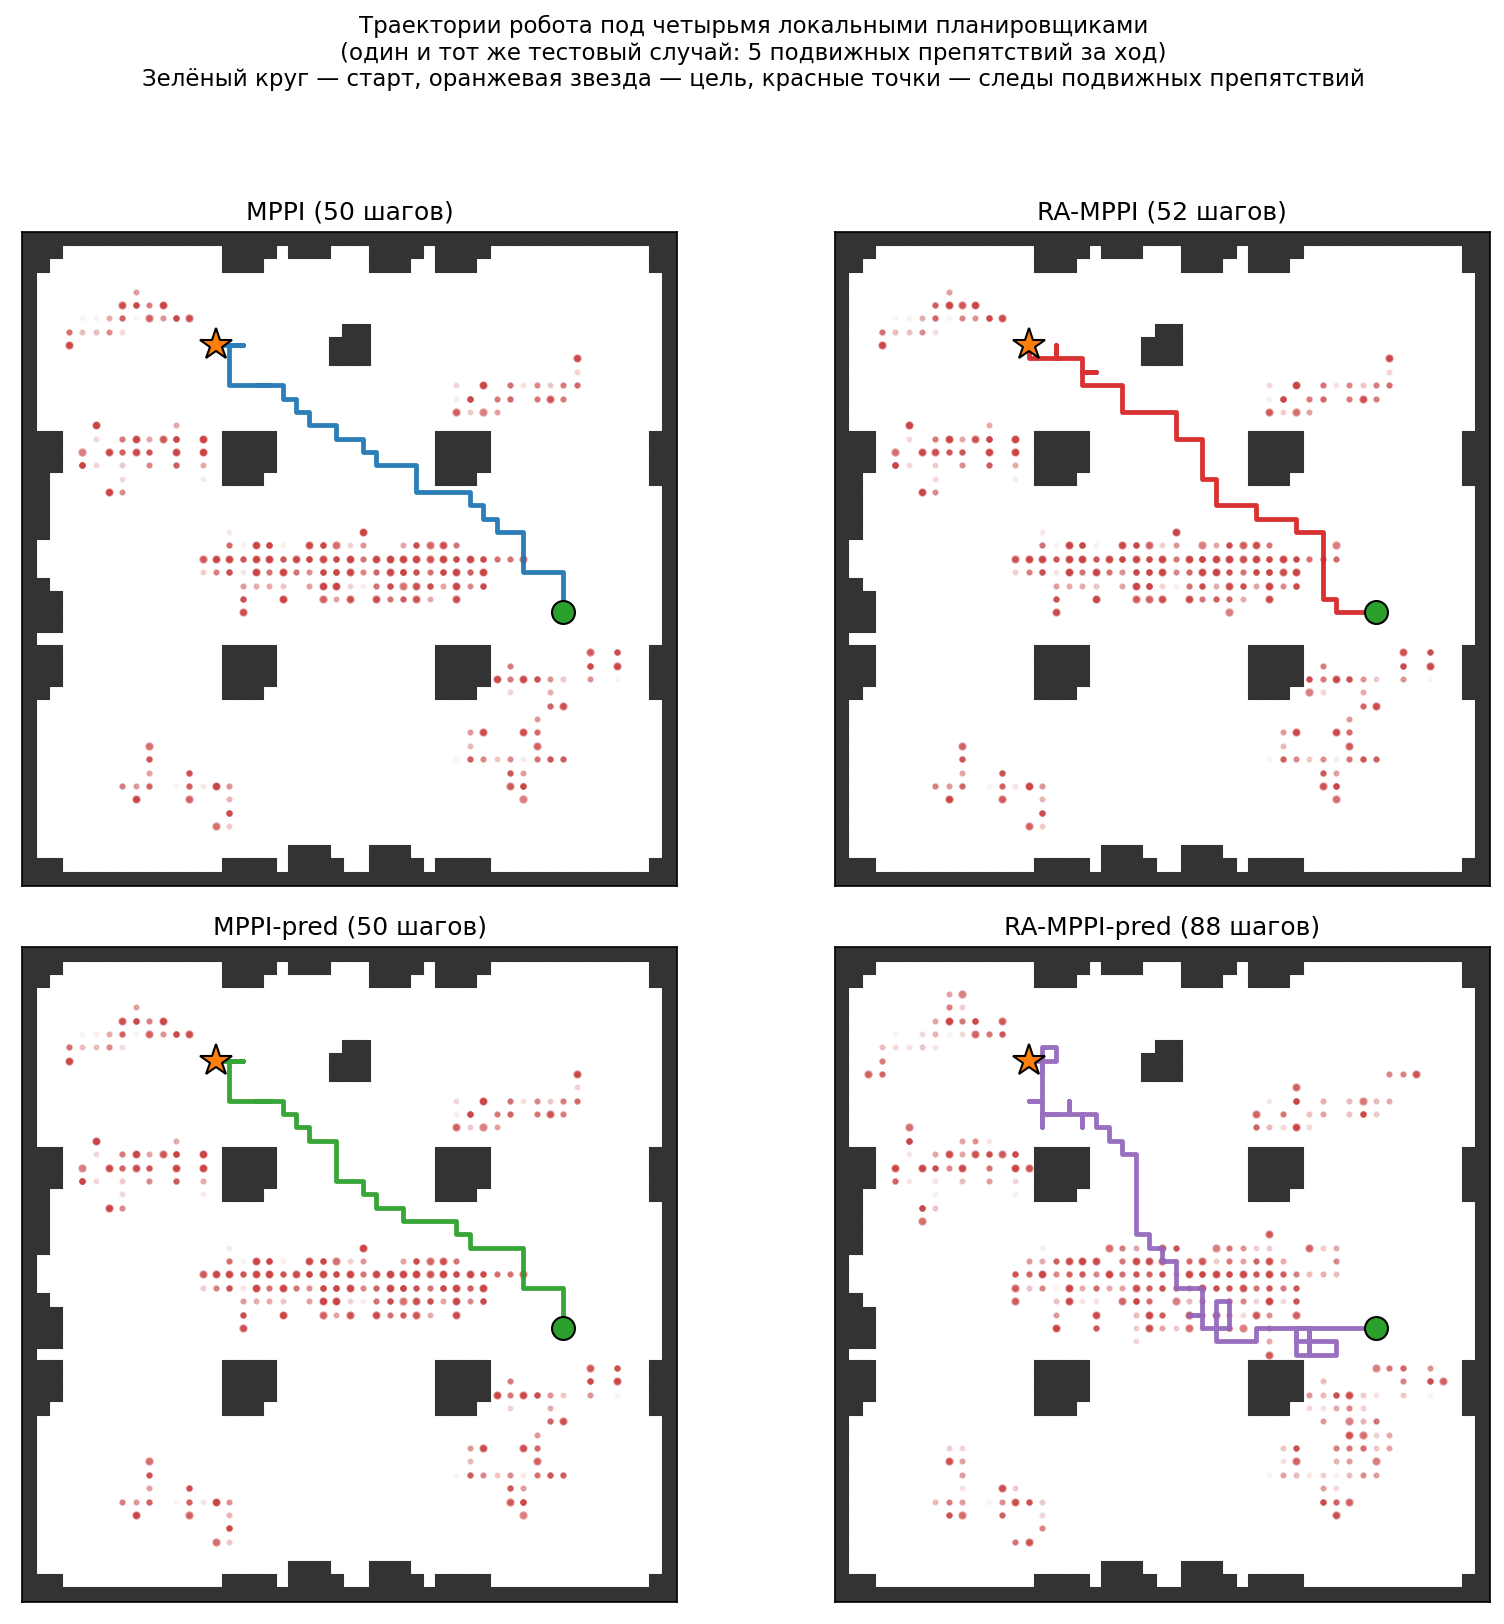
\includegraphics[width=0.92\textwidth]{trace_local_planners.png}
        \caption{Траектории робота под четырьмя локальными планировщиками на одном и том же тестовом случае (5 подвижных препятствий за ход): MPPI и MPPI-pred находят прямой маршрут, RA-MPPI отклоняется в сторону менее загруженной области, RA-MPPI-pred выбирает существенно более длинный обход.}
        \label{fig:trace_local_planners}
    \end{figure}

    \subsection{Анализ производительности в статической среде}

    В условиях неизменной карты MPPI и MPPI-pred решили по 96 задач из 100,
    RA-MPPI и RA-MPPI-pred --- по 94 (рис.~\ref{fig:local_static_comparison});
    остальные случаи зафиксированы как таймауты по ограничению в 500 шагов на задачу.
    При отсутствии подвижных препятствий список $\mathcal{D}$ пуст, поэтому MPPI-pred
    и RA-MPPI-pred вырождаются в свои базовые версии и должны воспроизводить их метрики
    с точностью до издержек ветвлений; полученные измерения это подтверждают.

    Для MPPI среднее время построения маршрута составило 15{,}07 мс, среднее число шагов --- 71{,}5,
    извилистость --- 2{,}267, доля опасных ситуаций --- 12{,}4\%.
    MPPI-pred показал практически идентичные показатели (15{,}48 мс, 71{,}5 шага, извилистость 2{,}267,
    доля опасных ситуаций 12{,}4\%), причём отличие в среднем времени укладывается в шум измерения.
    RA-MPPI занял заметно больше вычислительного бюджета --- 525{,}5 мс на задачу --- что
    объясняется вычислением CVaR по $N_d = 20$ возмущённым роллаутам для каждого из $K = 500$
    сэмплов; число шагов выросло до 84{,}8, извилистость --- до 2{,}643. Доля опасных ситуаций
    при этом снизилась более чем вдвое (5{,}4\% против 12{,}4\% у MPPI) благодаря тому,
    что CVaR-штраф вытесняет рискованные сэмплы из взвешенного среднего управления.
    RA-MPPI-pred повторил поведение RA-MPPI с точностью до измерения (539{,}3 мс, 84{,}8 шага,
    извилистость 2{,}643, доля опасных ситуаций 5{,}4\%).

    Полученная картина согласуется с теоретическим ожиданием: учёт хвостового риска повышает
    осторожность планировщика и увеличивает длину пути, но снижает частоту движений вблизи
    препятствий. Прогнозное слагаемое в статическом режиме не активируется и не влияет
    ни на качество траекторий, ни на бюджет вычислений.

    \subsection{Анализ производительности в динамической среде}

    Введение движущихся препятствий заметно меняет относительное поведение алгоритмов
    (рис.~\ref{fig:local_dynamic_comparison}). По всем трём уровням загрузки CVaR-варианты
    устойчиво превосходят базовый MPPI по доле опасных ситуаций, тогда как прогнозное
    слагаемое даёт наибольший вклад при умеренной плотности подвижных объектов.

    При одном объекте за ход MPPI решил 97 задач из 100, MPPI-pred --- 96, оба CVaR-варианта
    --- по 100. Снижение успешности базового MPPI объясняется поведением сэмплирующего
    планировщика в узких проходах: единственное движущееся препятствие может одновременно занять все
    соседние по горизонтали и вертикали клетки робота, и взвешенная сумма управлений приводит к
    выходу за пределы допустимых клеток. Прогнозное слагаемое в базовом MPPI на этой
    плотности не даёт устойчивого выигрыша по успешности, тогда как CVaR-штраф полностью
    парирует остаток отказов. Доля опасных ситуаций при разреженной динамике
    у MPPI-pred несколько ниже, чем у MPPI (17{,}6\% против 18{,}8\%), что согласуется
    с расширением запретной зоны вокруг предсказанной позиции. У RA-MPPI и RA-MPPI-pred
    доля опасных ситуаций составила 6{,}3\% и 6{,}8\% соответственно --- эффект прогноза
    перекрывается доминированием CVaR-штрафа и оказывается в пределах статистической погрешности.

    При пяти подвижных объектах все четыре варианта сохраняют близкую к 100\% успешность
    (RA-MPPI-pred --- 99\%). Длина пути и извилистость распределяются между парами
    «без прогноза / с прогнозом» неоднородно: у базового MPPI добавление прогноза
    практически не меняет геометрию траектории (64{,}8 против 65{,}6 шага, извилистость
    2{,}036 против 2{,}060), а доля опасных ситуаций даже несколько возрастает
    (17{,}5\% против 16{,}3\%). У RA-MPPI прогноз, напротив, заметно укорачивает путь
    (79{,}6 против 83{,}0 шага) и снижает долю опасных сближений (5{,}6\% против 6{,}4\%);
    эффект объясняется тем, что прогнозный штраф попадает в хвост распределения CVaR
    и более активно влияет на отбор безопасных траекторий, чем в базовой схеме softmin.

    При десяти подвижных объектах MPPI решил 98 задач из 100, MPPI-pred --- 100,
    RA-MPPI --- 100, RA-MPPI-pred --- 99. Доля опасных ситуаций распределилась как
    14{,}8\%, 15{,}3\%, 7{,}2\% и 8{,}3\% соответственно: переход от MPPI к RA-MPPI
    стабильно снижает долю опасных сближений приблизительно вдвое, тогда как добавление
    прогноза при высокой плотности динамики не даёт устойчивого выигрыша.
    Среднее число шагов и извилистость различаются в пределах 1--4\% между парами
    с прогнозом и без него.

    Стоимость прогноза по времени остаётся умеренной для базового MPPI: для одного,
    пяти и десяти объектов MPPI-pred требует 15{,}50, 13{,}47 и 16{,}07 мс соответственно
    против 15{,}62, 11{,}28 и 12{,}32 мс у MPPI; разница укладывается в пределах
    $\pm 30\%$ и колеблется в обе стороны из-за вариации длины траекторий.
    Для RA-MPPI-pred прогноз увеличивает время с 403{,}3 до 432{,}9 мс при $|\mathcal{D}| = 1$,
    с 395{,}0 до 473{,}2 мс при $|\mathcal{D}| = 5$ и с 394{,}0 до 553{,}5 мс при $|\mathcal{D}| = 10$,
    то есть на 7--40\%. Линейный рост согласуется с тем, что прогнозное слагаемое
    добавляет $O(K \cdot T \cdot |\mathcal{D}|)$ операций в номинальный роллаут
    и $O(N_d \cdot K \cdot T \cdot |\mathcal{D}|)$ в CVaR-цикл.

    \subsection{Выводы по главе}

    Проведённое сравнение четырёх вариантов локального планировщика выявило два
    принципиально различных рычага улучшения навигации: учёт хвостового риска (CVaR)
    и явный прогноз подвижных препятствий. Их вклад оказывается разной природы
    и плохо взаимозаменяем: CVaR преимущественно снижает долю опасных ситуаций
    и повышает успешность за счёт большей длины пути и значительной вычислительной
    стоимости, тогда как прогноз вносит локальную поправку, наиболее заметную
    при умеренной плотности подвижных объектов.

    \begin{table}[H]
        \centering
        \footnotesize
        \caption{Сравнительные характеристики MPPI, RA-MPPI и их prediction-вариантов}
        \label{tab:local_comparison}
        \begin{tabular}{|>{\raggedright\arraybackslash}p{0.30\textwidth}|
                         >{\centering\arraybackslash}p{0.13\textwidth}|
                         >{\centering\arraybackslash}p{0.13\textwidth}|
                         >{\centering\arraybackslash}p{0.13\textwidth}|
                         >{\centering\arraybackslash}p{0.13\textwidth}|}
            \hline
            \textbf{Параметр сравнения} & \textbf{MPPI} & \textbf{RA-MPPI} & \textbf{MPPI-pred} & \textbf{RA-MPPI-pred} \\
            \hline
            Статика: успешность & \textbf{96\%} & 94\% & \textbf{96\%} & 94\% \\
            \hline
            Статика: время, мс & \textbf{15{,}07} & 525{,}53 & 15{,}48 & 539{,}28 \\
            \hline
            Статика: число шагов & \textbf{71{,}5} & 84{,}8 & \textbf{71{,}5} & 84{,}8 \\
            \hline
            Статика: извилистость & \textbf{2{,}267} & 2{,}643 & \textbf{2{,}267} & 2{,}643 \\
            \hline
            Статика: доля опасных ситуаций & 12{,}4\% & \textbf{5{,}4\%} & 12{,}4\% & \textbf{5{,}4\%} \\
            \hline\hline
            Динамика (1): успешность & 97\% & \textbf{100\%} & 96\% & \textbf{100\%} \\
            \hline
            Динамика (1): время, мс & 15{,}62 & 403{,}27 & \textbf{15{,}50} & 432{,}94 \\
            \hline
            Динамика (1): число шагов & 88{,}4 & 84{,}7 & \textbf{84{,}0} & 85{,}8 \\
            \hline
            Динамика (1): извилистость & 2{,}845 & 2{,}683 & \textbf{2{,}675} & 2{,}744 \\
            \hline
            Динамика (1): доля опасных ситуаций & 18{,}8\% & \textbf{6{,}3\%} & 17{,}6\% & 6{,}8\% \\
            \hline\hline
            Динамика (5): успешность & \textbf{100\%} & \textbf{100\%} & \textbf{100\%} & 99\% \\
            \hline
            Динамика (5): время, мс & \textbf{11{,}28} & 394{,}95 & 13{,}47 & 473{,}16 \\
            \hline
            Динамика (5): число шагов & \textbf{64{,}8} & 83{,}0 & 65{,}6 & 79{,}6 \\
            \hline
            Динамика (5): извилистость & \textbf{2{,}036} & 2{,}587 & 2{,}060 & 2{,}542 \\
            \hline
            Динамика (5): доля опасных ситуаций & 16{,}3\% & 6{,}4\% & 17{,}5\% & \textbf{5{,}6\%} \\
            \hline\hline
            Динамика (10): успешность & 98\% & \textbf{100\%} & \textbf{100\%} & 99\% \\
            \hline
            Динамика (10): время, мс & \textbf{12{,}32} & 393{,}99 & 16{,}07 & 553{,}48 \\
            \hline
            Динамика (10): число шагов & 68{,}3 & 80{,}3 & \textbf{67{,}1} & 83{,}1 \\
            \hline
            Динамика (10): извилистость & 2{,}135 & 2{,}505 & \textbf{2{,}109} & 2{,}632 \\
            \hline
            Динамика (10): доля опасных ситуаций & 14{,}8\% & \textbf{7{,}2\%} & 15{,}3\% & 8{,}3\% \\
            \hline
        \end{tabular}
    \end{table}

    \clearpage

    Полученные данные показывают, что переход от MPPI к RA-MPPI снижает долю опасных
    ситуаций в 2--3 раза в зависимости от плотности динамики, но увеличивает время
    планирования примерно в 30 раз ($\approx 13$ мс против $\approx 430$ мс) и удлиняет
    путь от $-4\%$ (разреженная динамика) до $+28\%$ (статика и средняя динамика).
    Прогнозное слагаемое, напротив, вносит более скромные изменения: для базового MPPI
    оно колеблется в пределах $\pm 1{,}5$ процентного пункта по доле опасных ситуаций
    и заметного устойчивого выигрыша по геометрии траектории не показывает.
    Для RA-MPPI прогноз даёт наиболее выраженный эффект при средней плотности
    подвижных объектов: укорачивает путь и снижает долю опасных сближений
    на $0{,}8$ процентного пункта при пяти препятствиях за ход, но при разреженной
    и плотной динамике его вклад в долю опасных ситуаций оказывается в пределах
    статистической погрешности, проявляясь главным образом в виде дополнительного времени вычислений.

    Таким образом, выбор конкретной комбинации остаётся компромиссом между допустимой
    вычислительной задержкой и требуемым уровнем безопасности.
    MPPI пригоден как минимально нагрузочный вариант для разреженных сред с редко
    возникающими подвижными препятствиями. MPPI-pred представляет собой малозатратное
    расширение, дающее выигрыш на промежуточных режимах динамики без существенного роста
    вычислительной стоимости. RA-MPPI предпочтителен там, где приоритетом является
    интерпретируемое снижение хвостового риска, а вычислительный бюджет позволяет
    оплатить $N_d$-кратное расширение объёма роллаутов. RA-MPPI-pred оправдан только тогда,
    когда от системы требуется одновременно учёт хвостового риска и явный прогноз;
    в исследованной случайно-блуждающей модели среды его дополнительный выигрыш
    по сравнению с RA-MPPI находится на грани статистической значимости.

    \pagebreak

    \section{Реализация навигационного стека в ROS\,2 и сквозное тестирование}
    \label{sec:ros-impl}

    В предыдущих главах исследование выполнялось в виде самостоятельных программных
    моделей, фокусирующихся на отдельных метриках выбранных алгоритмов: скорости перепланирования
    для $A^*/D^*$\,Lite и качестве траекторий для MPPI/RA-MPPI\@.
    Цель настоящей главы --- интегрировать эти алгоритмы в единый навигационный стек
    и подтвердить их совместную работоспособность на физическом симуляторе мобильного робота.

    \subsection{Архитектура и используемые компоненты}

    Реализация выполнена на стеке ROS\,2 Jazzy с физическим симулятором
    Gazebo Sim Harmonic (gz-sim) и фреймворком навигации Nav2.
    В качестве робота выбран TurtleBot3 Burger --- двухколёсная дифференциальная
    платформа радиусом 10\,см с лазерным сканером 360\textdegree, что соответствует
    типичной конфигурации мобильных роботов в логистике.

    Архитектура построена на модели <<глобальный планировщик + локальный контроллер>>,
    разделение которой обосновано в главе~\ref{sec:review}.
    Глобальный уровень получает на вход карту занятости и текущее положение робота
    и выдаёт опорный путь до цели; локальный уровень преобразует опорный путь
    в управляющие команды по линейной и угловой скорости, реагируя на показания сенсоров
    и движущиеся объекты.

    Все четыре исследуемых конфигурации строятся комбинированием двух глобальных планировщиков -- классического $A^*$, реализованного штатным модулем графового поиска пути Nav2, и собственной реализации $D^*$\,Lite, оформленной как отдельный плагин стека, -- с двумя локальными контроллерами: штатным MPPI из дистрибутива Nav2 и собственной реализацией RA-MPPI, также оформленной как плагин.

    Соответствие каждой пары планировщик-контроллер фиксируется отдельным конфигурационным файлом параметров Nav2. Общая структура такого файла включает узел глобального планирования, узел локального управления, узел поведенческих стратегий и исполнитель дерева поведений, который переключает робота между режимом обычной навигации и режимами восстановления; два слоя карты затрат -- глобальный, отражающий известную карту окружения, и локальный, ограниченный окрестностью робота и обновляемый по показаниям сенсоров; а также стандартный набор узлов восстановления (поворот на месте, кратковременный отход назад, ожидание).

    \subsection{Разработанные программные пакеты}

    В составе работы реализованы два собственных пакета ROS\,2 и набор вспомогательных
    скриптов для построения экспериментов и анализа bag-файлов.

    \subsubsection{Реализация D*\,Lite в виде плагина Nav2}

    Пакет реализует $D^*$\,Lite в виде глобального планировщика-плагина Nav2 и состоит из четырёх логических частей. Первая часть -- ядро алгоритма: обновление одношаговых $\mathit{rhs}$-оценок, очередь приоритетов с двухключевой схемой $D^*$\,Lite, перерасчёт изменившихся вершин. Вторая часть отвечает за преобразование локальной карты затрат, поддерживаемой Nav2, в граф 4-связности с отсечением клеток выше порога летальной стоимости. Третья часть реализует манхэттенскую эвристику $h(s) = |s_x - g_x| + |s_y - g_y|$, допустимую при равных весах рёбер 4-связного графа. Четвёртая часть -- адаптерный слой плагина: жизненный цикл внутри стека Nav2, извлечение актуальной карты затрат при каждом запросе планирования и конвертация результата во внутренний формат пути. Возникающие на диагональных участках лестничные траектории сглаживаются локальным контроллером в рамках штрафа выравнивания пути и pure-pursuit-цели без существенного замедления движения.

    Внутри ядра $D^*$\,Lite сохранены все инкрементальные свойства, ранее подтверждённые в главе~3. Однако в рамках Nav2-плагина каждый вызов планирования заново строит граф и запускает алгоритм от текущего состояния карты: интерфейс глобального планировщика Nav2 не передаёт сведений о том, какие именно ячейки карты изменились между вызовами, а само перепланирование инициируется самим стеком по таймеру с фиксированной частотой. В рассматриваемых сценариях это не сказывается на качестве траекторий: карта компактна ($112 \times 103$ ячеек), полный поиск занимает единицы миллисекунд и сопоставим по времени с накладными расходами Nav2 на формирование результата.

    \subsubsection{Реализация RA-MPPI в виде плагина Nav2}

    Пакет реализует RA-MPPI в виде локального контроллера-плагина Nav2. Ядро алгоритма воспроизводит реализацию модельного эксперимента из главы~4: $K$ номинальных траекторий, оценка функции стоимости, для каждой траектории --- $N_d$ возмущённых роллаутов с дополнительным шумом $\sigma_d$, вычисление CVaR$_\alpha$ и добавление штрафа $\gamma \cdot \text{CVaR}$, затем стандартное взвешивание Больцмана по скорректированным стоимостям.

    Адаптерный слой реализует интерфейсный слой ROS\,2: подписку на текущий глобальный путь, преобразование между системами координат карты и одометрии робота, формирование команды по линейной и угловой скорости и проверку достижения цели; локальный кэш карты затрат используется для быстрой проверки столкновений сэмплируемых траекторий. Прямое использование первой точки глобального плана как промежуточной цели приводило к колебаниям контроллера у криволинейных участков пути, поэтому применён классический метод pure-pursuit -- стандартный приём следования по пути в робототехнике, в котором робот ориентируется не на ближайшую к нему точку плана, а на так называемую \emph{опорную точку} (look-ahead point), расположенную впереди него на фиксированном расстоянии $L_{\text{lookahead}}$ вдоль глобального пути; именно эта опорная точка и используется в качестве цели MPPI. Значение $L_{\text{lookahead}} = 0{,}80$\,м даёт компромисс между предсказательной способностью и агрессивностью отклонений от глобального плана.

    Значения параметров пучка траекторий, использованные в главе~4 ($K = 500$, $\sigma = 0{,}8$), в условиях полной системы Nav2 не укладываются в целевой бюджет такта контроллера (100\,мс при частоте $10$\,Гц): уже один проход MPPI на $K = 500$ сэмплах при горизонте $T = 12$ занимает порядка десятков миллисекунд, а с учётом построения карты затрат, преобразований систем координат и публикации команд суммарное время выходит за рамки бюджета. В ROS-реализации число сэмплов уменьшено до $K = 150$, а стандартное отклонение шума управления увеличено до $\sigma = 1{,}0$, что сохраняет необходимую ширину пучка управлений при существенно меньшем числе траекторий и не приводит к преждевременной концентрации весов Больцмана на узкой группе сэмплов.

    \subsection{Среда тестирования и сценарии}

    Базовая карта --- стандартный мир \texttt{turtlebot3\_world}, представляющий
    собой квадрат $4{,}2 \times 4{,}0$\,м, ограниченный стенами,
    с регулярной сеткой $3{\times}3$ цилиндрических колонн радиусом 15\,см.
    Все эксперименты используют общий маршрут:
    старт $(-2{,}0,\,-0{,}5)$, цель $(1{,}8,\,0{,}5)$,
    что соответствует диагональному пересечению карты с прохождением через
    верхний коридор (между северным рядом колонн и стеной).
    Базовая карта показана на рисунке~\ref{fig:map_static}: зелёный круг ---
    точка старта, красный --- цель.

    \begin{figure}[H]
        \centering
        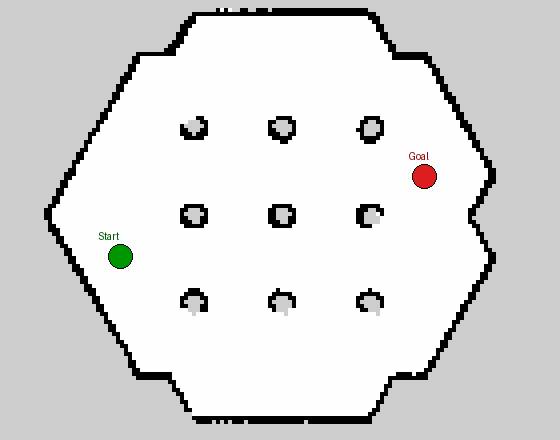
\includegraphics[width=0.55\textwidth]{map_static.png}
        \caption{Статическая карта \texttt{turtlebot3\_world}: $3{\times}3$
        колонн, старт $(-2{,}0;\,-0{,}5)$, цель $(1{,}8;\,0{,}5)$.}
        \label{fig:map_static}
    \end{figure}

    Для оценки устойчивости к движущимся препятствиям сгенерированы три
    динамических мира:
    \texttt{dynamic\_1} (одно препятствие, целенаправленно пересекающее траекторию),
    \texttt{dynamic\_5} (умеренная плотность, 5 препятствий),
    \texttt{dynamic\_10} (высокая плотность, 10 препятствий).
    Каждое препятствие движется кинематически по синусоиде вдоль своего коридора.
    В сценариях \texttt{dynamic\_1} и \texttt{dynamic\_5} все цилиндры используют
    единые параметры (период 17\,с, амплитуда 0{,}55\,м), что обеспечивает
    пиковую скорость 0{,}20\,м/с. В сценарии \texttt{dynamic\_10} периоды
    варьируются в диапазоне 12--20\,с, амплитуды --- в диапазоне 0{,}35--0{,}55\,м,
    что даёт пиковые скорости 0{,}13--0{,}21\,м/с и моделирует более разнородную
    динамическую среду. Указанный диапазон скоростей сопоставим с целевой
    скоростью робота ($\sim$0{,}25\,м/с) и позволяет локальному контроллеру в
    принципе предсказать траекторию препятствия на горизонте планирования.
    Расположение цилиндров и их коридоры движения для трёх плотностей
    показаны на рисунке~\ref{fig:map_dynamic}: синие круги ---
    начальные позиции, светло-синие линии --- допустимые отрезки
    синусоидального движения.

    \begin{figure}[H]
        \centering
        \begin{subfigure}[t]{0.31\textwidth}
            \centering
            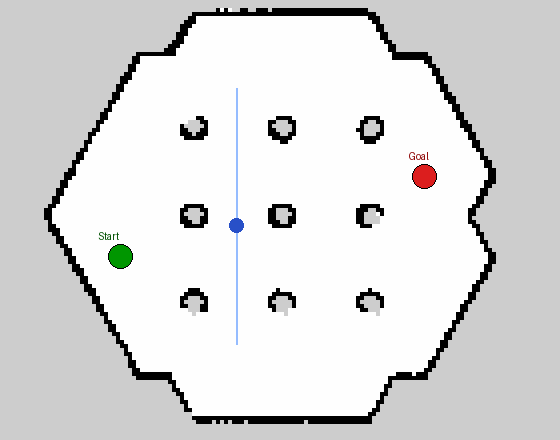
\includegraphics[width=\linewidth]{map_dynamic_1.png}
            \caption{\texttt{dynamic\_1}}\label{fig:map_d1}
        \end{subfigure}\hfill
        \begin{subfigure}[t]{0.31\textwidth}
            \centering
            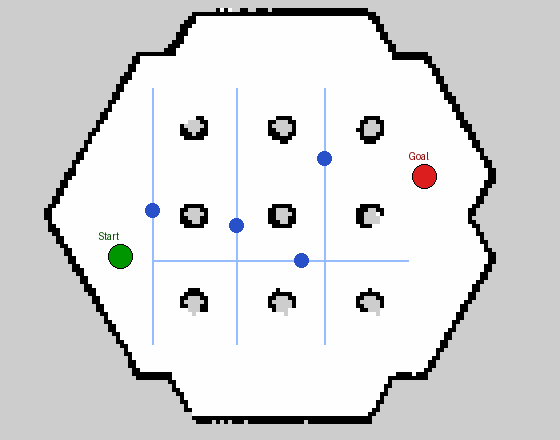
\includegraphics[width=\linewidth]{map_dynamic_5.png}
            \caption{\texttt{dynamic\_5}}\label{fig:map_d5}
        \end{subfigure}\hfill
        \begin{subfigure}[t]{0.31\textwidth}
            \centering
            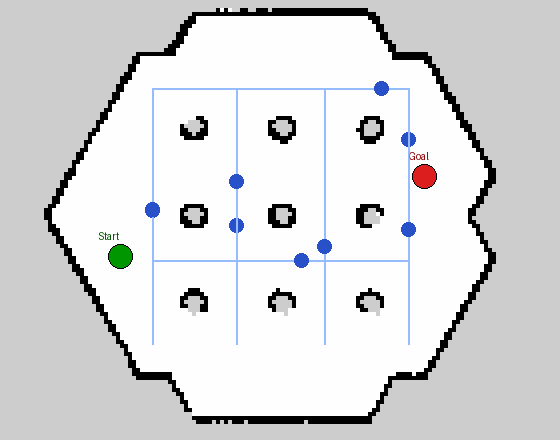
\includegraphics[width=\linewidth]{map_dynamic_10.png}
            \caption{\texttt{dynamic\_10}}\label{fig:map_d10}
        \end{subfigure}
        \caption{Карты с подвижными цилиндрическими препятствиями.}
        \label{fig:map_dynamic}
    \end{figure}

    На каждом сценарии фиксируются пять метрик:
    \textit{успешность} --- достиг ли робот окрестности цели (толерантность 0{,}35\,м)
    в пределах 120-секундного бюджета;
    \textit{итоговое отклонение} --- расстояние от финальной точки робота до цели;
    \textit{длина пути} --- суммарное смещение по одометрии;
    \textit{длительность} --- время от первого до последнего сообщения о позе робота;
    \textit{опасные сближения} --- число эпизодов, когда штатный модуль контроля безопасности Nav2 регистрировал критически малую дистанцию между роботом и ближайшим препятствием (как статическим, так и подвижным) и принудительно тормозил или останавливал робот; последовательные срабатывания, разделённые паузой менее 2\,с, объединяются в одно событие, чтобы не учитывать дважды одну и ту же опасную ситуацию.

    Подвижные препятствия перемещаются по карте кинематически (без физического моделирования контактов): каждый цилиндр имеет заранее назначенную синусоидальную траекторию вдоль своего коридора и обновляет позицию с частотой 10\,Гц.

    Логика движения дополнена поведенческим условием: цилиндр не вытесняет робот. Запланированная позиция вычисляется заранее, и если она попадает в зону безопасности радиуса $0{,}30$\,м вокруг робота, цилиндр временно удерживается на текущей координате и не смещается в сторону робота. Такое поведение сохраняет реалистичность твёрдого неподвижного препятствия и требует от локального контроллера активного объезда.

    \subsection{Линейное предсказание траекторий динамических препятствий}

    Штатный MPPI-контроллер из дистрибутива Nav2 не различает статические и динамические препятствия: стоимость роллаута определяется по текущей карте затрат, которая обновляется лишь на следующем цикле Nav2. Для конфигураций с собственным контроллером RA-MPPI (пары $A^*$+RA-MPPI и $D^*$\,Lite+RA-MPPI) реализовано линейное предсказание положений цилиндров непосредственно внутри оценщика стоимости роллаутов. Конфигурации со штатным MPPI-контроллером предсказания не выполняют и воспринимают движущиеся цилиндры как статические объекты, сместившиеся к текущему обновлению карты затрат.

    Передача состояний цилиндров между процессом перемещения цилиндров и контроллером реализована через общий файл, обновляемый на каждом такте (10\,Гц): для каждого цилиндра записывается его текущая позиция $(x, y)$ и аналитическая скорость $(v_x, v_y)$. Скорость вычисляется как производная заданной синусоиды: $v = A \cdot \tfrac{2\pi}{T} \cos\!\bigl(\tfrac{2\pi}{T}t + \varphi\bigr)$. Контроллер RA-MPPI перед каждым запросом очередного шага считывает этот файл и переводит мировые координаты в координаты ячейки карты затрат стандартными средствами Nav2:
    \[
        \mathit{row} = \frac{y_w - o_y}{\Delta},\quad
        \mathit{col} = \frac{x_w - o_x}{\Delta},\quad
        v_{\mathit{row}} = \frac{v_y}{\Delta},\quad
        v_{\mathit{col}} = \frac{v_x}{\Delta},
    \]
    где $\Delta$ --- разрешение карты затрат (м/ячейку), $(o_x, o_y)$ --- координаты начала карты в мировой системе координат.

    В каждом шаге роллаута $t$ вычисляется предсказанное положение препятствия:
    \[
        p_{\mathit{row}}(t) = \mathit{row} + v_{\mathit{row}} \cdot t \cdot \Delta t,\quad
        p_{\mathit{col}}(t) = \mathit{col} + v_{\mathit{col}} \cdot t \cdot \Delta t,
    \]
    и к стоимости роллаута добавляется штраф:
    \[
        c_{\mathrm{obs}}(t) =
        \begin{cases}
            c_{\mathrm{hard}}, & d(t) < r_{\mathrm{hard}},\\
            c_{\mathrm{soft}}\,\bigl(1 - d(t)/r_{\mathrm{soft}}\bigr)^2, & r_{\mathrm{hard}} \le d(t) < r_{\mathrm{soft}},\\
            0, & \text{иначе},
        \end{cases}
    \]
    где $d(t)$ --- расстояние от позиции роллаута до предсказанного центра цилиндра. В RA-MPPI тот же штраф применяется в обоих типах роллаутов: номинальных (для оценки средней стоимости) и возмущённых (для вычисления CVaR-хвоста), что позволяет оценивать риск столкновения с движущимся препятствием с учётом неопределённости управления.

    Параметры штрафа: жёсткий радиус $r_{\mathrm{hard}} = (r_{\mathrm{cyl}} + m_{\mathrm{hard}}) / \Delta$ ($r_{\mathrm{cyl}} = 0{,}15$\,м --- радиус цилиндра, $m_{\mathrm{hard}} = 0{,}09$\,м --- запас), мягкий $r_{\mathrm{soft}} = 0{,}70$\,м/$\Delta$.

    \subsection{Результаты экспериментов}

    Тестирование выполнено на 16 сценариях --- декартово произведение четырёх комбинаций \textit{планировщик--контроллер} и четырёх миров. Каждый сценарий запускался 10 раз независимо; на каждом прогоне поднимался независимый экземпляр Gazebo, Nav2 и процесса перемещения цилиндров, bag-файл записывался полностью и анализировался Python-скриптом пост-обработки. Фиксировалось число успешных и неудачных попыток, а метрические показатели усреднялись по успешным прогонам.

    Сводные результаты приведены в таблице~\ref{tab:ros_full}. Колонка \textit{Планировщик} обозначает комбинацию глобального планировщика и локального контроллера (один из $A^*$ / $D^*$\,Lite в паре с одним из MPPI / RA-MPPI); колонка \textit{Мир} --- тестовый сценарий: \textit{static} (без подвижных препятствий) или \textit{dynamic\_N} (мир с $N$ движущимися цилиндрами). Колонки \textit{Усп.} и \textit{Неуд.} содержат число успешных и неудачных прогонов из десяти; успешным считается прогон, в котором робот достиг окрестности цели с толерантностью 0{,}35\,м за 120\,с. Колонка \textit{Откл., м} --- среднее расстояние от финальной точки робота до цели по успешным прогонам; \textit{Путь, м} --- средняя суммарная длина траектории по данным одометрии; \textit{Время, с} --- средняя длительность теста от первой до последней опубликованной позы робота. Колонка \textit{Сбл.} приводит среднее число срабатываний штатного модуля контроля безопасности Nav2, разделённых паузой более 2\,с, и отражает частоту принудительных торможений из-за динамических препятствий.

    \begin{table}[H]
        \centering
        \footnotesize
        \caption{Результаты сквозного тестирования навигационного стека ROS\,2 / Nav2 (10 прогонов на сценарий).}
        \label{tab:ros_full}
        \begin{tabular}{|l|l|c|c|c|c|c|c|}
            \hline
            \textbf{Планировщик} & \textbf{Мир} &
            \textbf{Усп.} & \textbf{Неуд.} &
            \textbf{Откл., м} & \textbf{Путь, м} & \textbf{Время, с} & \textbf{Сбл.} \\
            \hline
            $A^*$    + MPPI       & static      & \textbf{10} & \textbf{0} & 0{,}252 & \textbf{4{,}21} & 18{,}1 & \textbf{0{,}00} \\\hline
            $D^*$\,Lite + MPPI    & static      & \textbf{10} & \textbf{0} & 0{,}254 & 4{,}46 & 21{,}4 & \textbf{0{,}00} \\\hline
            $A^*$    + RA-MPPI    & static      & \textbf{10} & \textbf{0} & \textbf{0{,}190} & 4{,}47 & 18{,}7 & \textbf{0{,}00} \\\hline
            $D^*$\,Lite + RA-MPPI & static      & \textbf{10} & \textbf{0} & 0{,}245 & 4{,}45 & \textbf{16{,}6} & \textbf{0{,}00} \\\hline\hline
            $A^*$    + MPPI       & dynamic\_1  & \textbf{10} & \textbf{0} & 0{,}240 & \textbf{4{,}25} & 19{,}3 & \textbf{0{,}00} \\\hline
            $D^*$\,Lite + MPPI    & dynamic\_1  & \textbf{10} & \textbf{0} & 0{,}262 & 4{,}47 & 21{,}8 & 0{,}10 \\\hline
            $A^*$    + RA-MPPI    & dynamic\_1  & \textbf{10} & \textbf{0} & \textbf{0{,}180} & 4{,}62 & 22{,}6 & \textbf{0{,}00} \\\hline
            $D^*$\,Lite + RA-MPPI & dynamic\_1  & \textbf{10} & \textbf{0} & 0{,}237 & 4{,}49 & \textbf{18{,}0} & \textbf{0{,}00} \\\hline\hline
            $A^*$    + MPPI       & dynamic\_5  &  9 & 1 & 0{,}238 & 4{,}78 & 30{,}7 & 0{,}30 \\\hline
            $D^*$\,Lite + MPPI    & dynamic\_5  & \textbf{10} & \textbf{0} & 0{,}254 & \textbf{4{,}51} & 22{,}1 & \textbf{0{,}00} \\\hline
            $A^*$    + RA-MPPI    & dynamic\_5  & \textbf{10} & \textbf{0} & \textbf{0{,}194} & 4{,}91 & 22{,}2 & \textbf{0{,}00} \\\hline
            $D^*$\,Lite + RA-MPPI & dynamic\_5  & \textbf{10} & \textbf{0} & 0{,}221 & 4{,}58 & \textbf{19{,}4} & \textbf{0{,}00} \\\hline\hline
            $A^*$    + MPPI       & dynamic\_10 & \textbf{10} & \textbf{0} & 0{,}221 & 4{,}84 & 41{,}9 & 1{,}00 \\\hline
            $D^*$\,Lite + MPPI    & dynamic\_10 & \textbf{10} & \textbf{0} & 0{,}258 & \textbf{4{,}55} & 24{,}3 & \textbf{0{,}00} \\\hline
            $A^*$    + RA-MPPI    & dynamic\_10 & \textbf{10} & \textbf{0} & \textbf{0{,}148} & 5{,}26 & 27{,}3 & 0{,}20 \\\hline
            $D^*$\,Lite + RA-MPPI & dynamic\_10 &  9 & 1 & 0{,}209 & 4{,}90 & \textbf{23{,}6} & 0{,}22 \\\hline
        \end{tabular}
    \end{table}

    В статическом мире все четыре конфигурации справляются со 100\,\% успешностью.
    Быстрейшим оказывается $D^*$\,Lite\,+\,RA-MPPI (16{,}6\,с), $A^*$\,+\,MPPI
    и $A^*$\,+\,RA-MPPI сопоставимы (18{,}1 и 18{,}7\,с), тогда как
    $D^*$\,Lite\,+\,MPPI немного медленнее (21{,}4\,с).
    Длина пути варьируется в узком диапазоне 4{,}2--4{,}5\,м, что
    подтверждает малозначимость выбора глобального планировщика для
    метрики пути в простых условиях.

    При наличии одного движущегося цилиндра (\texttt{dynamic\_1}) все конфигурации
    также достигают 100\,\% успешности; порядок скоростей сохраняется:
    $D^*$\,Lite\,+\,RA-MPPI лидирует (18{,}0\,с), $A^*$\,+\,MPPI и
    $A^*$\,+\,RA-MPPI — 19{,}3 и 22{,}6\,с, $D^*$\,Lite\,+\,MPPI — 21{,}8\,с.
    Единичное срабатывание модуля контроля безопасности у $D^*$\,Lite\,+\,MPPI (0{,}10)
    отражает то, что инкрементальный планировщик реже уводит робота
    в обход, вынуждая локальный контроллер тормозить.

    В сценарии \texttt{dynamic\_5} впервые проявляется нестабильность
    $A^*$\,+\,MPPI: 9 успешных прогонов из 10, среднее время на успешных
    прогонах — 30{,}7\,с, среднее число сближений — 0{,}30.
    Остальные три конфигурации сохраняют 100\,\% успешность при времени
    19--22\,с. Неудача $A^*$\,+\,MPPI воспроизводится стабильно
    (подтверждена повторными прогонами): при плотном расположении пяти
    цилиндров MPPI-контроллер с эвристикой $A^*$ периодически попадает
    в тупиковое локальное оптимальное состояние, из которого не может
    выйти за 120\,с.

    В наиболее сложном сценарии \texttt{dynamic\_10} контраст между
    конфигурациями максимален. $A^*$\,+\,MPPI остаётся полностью
    успешным (10/10), однако ценой резкого роста времени (41{,}9\,с) и
    высокого числа сближений (1{,}00 за прогон): контроллер многократно
    тормозит из-за движущихся цилиндров. $D^*$\,Lite\,+\,MPPI
    справляется значительно быстрее (24{,}3\,с) при нулевых сближениях —
    инкрементальное перепланирование позволяет заблаговременно
    обойти динамические объекты. $A^*$\,+\,RA-MPPI показывает 27{,}3\,с
    при 0{,}20 сближениях: CVaR-штраф удерживает робота от опасной
    близости, однако без глобального перепланирования траектория длиннее.
    $D^*$\,Lite\,+\,RA-MPPI даёт 9/10 (23{,}6\,с, 0{,}22 сближения):
    один неудачный прогон вызван блокировкой сразу несколькими цилиндрами,
    после чего навигация не укладывалась в таймаут.

    Финальное отклонение от цели по успешным прогонам составляет
    0{,}15--0{,}26\,м во всех сценариях, что существенно меньше
    порога 0{,}35\,м и свидетельствует о стабильной точности
    позиционирования независимо от сложности среды.

    \subsection{Выводы по главе}

    Эксперименты показали, что исследованные в главах~3--4 алгоритмы успешно
    работают в составе целевой инженерной системы --- ROS\,2 / Nav2 / Gazebo Sim.
    Сборка и стабилизация интегрированного стека потребовала разработки
    двух собственных пакетов (\texttt{dstar\_lite\_planner},
    \texttt{ramppi\_controller}), кинематического модуля перемещения
    препятствий и набора скриптов оркестрации тестов и пост-обработки.
    Из 16 сценариев 14 завершились со 100\,\% успешностью; единственные
    исключения --- $A^*$\,+\,MPPI в \texttt{dynamic\_5} (9/10)
    и $D^*$\,Lite\,+\,RA-MPPI в \texttt{dynamic\_10} (9/10) ---
    отражают реальную сложность навигации при высокой плотности
    движущихся препятствий, а не дефекты реализации.
    Наиболее стабильной и быстрой во всех динамических мирах
    оказывается связка $D^*$\,Lite\,+\,MPPI, сочетающая инкрементальное
    перепланирование с нулевыми сближениями при dynamic\_10;
    $D^*$\,Lite\,+\,RA-MPPI демонстрирует наименьшее время в статичных
    и малодинамичных сценариях (16{,}6 и 18{,}0\,с).

    \newpage

    \section*{Описание применения генеративной модели}
    \addcontentsline{toc}{section}{Описание применения генеративной модели}

    При выполнении работы в качестве вспомогательного инструмента
    применялась генеративная модель Claude Opus~4.8 (компания Anthropic).
    Доступ к модели осуществлялся через её официальный сайт
    \url{https://claude.ai} и интерфейс командной строки \texttt{Claude Code}.

    Целями применения модели: редактирование текста работы
    и тестирование разработанного программного кода. 
    При редактировании текста модель использовалась для устранения
    стилистических и грамматических неточностей и повышения связности изложения. 
    При тестировании программного кода модель привлекалась для проверки
    работоспособности реализованных компонентов и выявления ошибок в ходе
    запуска тестов.

    По способу применения взаимодействие велось в интерактивном диалоговом
    режиме: описывалась задача и место, которое требовалось
    проверить, после чего модель предлагала правки; предложенные правки
    изучались, проверялись вручную и на их основе редактировался текст или код.

    \newpage

    \section*{Заключение}
    \addcontentsline{toc}{section}{Заключение}

    В рамках курсовой работы решена комплексная задача исследования и
    практической реализации алгоритмов навигации мобильного робота
    в статической и динамической среде.

    В аналитической части выполнен систематический обзор современных методов глобального и локального планирования. Рассмотрены графовые, сэмплирующие и бионические глобальные планировщики, а также классические контроллеры, геометрические и оптимизационные методы локального управления. На основе сравнительного анализа обоснован выбор $D^*$\,Lite в качестве глобального планировщика, обеспечивающего инкрементальное перепланирование при локальных изменениях карты. На уровне локального управления для последующего экспериментального сравнения отобраны MPPI и RA-MPPI --- стохастические предсказательные контроллеры, способные работать с нелинейной динамикой и учитывать препятствия через функцию стоимости.

    Для экспериментального сравнения глобальных планировщиков разработана
    собственная программная модель на C++ и проведено сравнение $A^*$ и
    $D^*$\,Lite на модифицированной карте <<Arena>> ($49\times 49$ клеток) при 1000
    случайных задачах на каждую конфигурацию. Показано, что в статической
    среде $A^*$ остаётся оптимальным выбором благодаря лёгкому однократному
    поиску ($0{,}22$--$0{,}74$\,мс против $1{,}26$--$5{,}69$\,мс у $D^*$\,Lite),
    однако в режиме высокой динамики (15 препятствий за ход)
    $D^*$\,Lite сокращает время обновления пути в $12$--$15$ раз
    ($\sim 1$--$9$\,мс против $\sim 2$--$156$\,мс), что делает его единственным
    масштабируемым решением для систем реального времени.

    На той же модели проведено сравнение локальных контроллеров MPPI и RA-MPPI на 100 навигационных задачах. RA-MPPI реализует мягкий CVaR-штраф на основе возмущённых роллаутов и устойчиво превосходит MPPI по доле опасных сближений с препятствиями (в несколько раз ниже во всех режимах динамики), а также показывает несколько более высокую успешность в плотных сценариях. Платой за это становится значительный рост вычислительных затрат, обусловленный дополнительным внутренним циклом по возмущённым роллаутам в CVaR-оценке.

    На этапе практической реализации алгоритмы интегрированы в навигационный
    стек ROS\,2 / Nav2 / Gazebo Sim в виде двух собственных плагинов:
    глобального планировщика $D^*$\,Lite и локального контроллера RA-MPPI.
    Дополнительно разработаны модуль кинематического перемещения цилиндров
    и набор скриптов оркестрации экспериментов. На сквозном
    бенчмарке из 16 сценариев (4 пары планировщик--контроллер на 4 мирах
    с числом подвижных препятствий $0$--$10$, по 10 прогонов на каждый
    сценарий) подтверждена совместная работоспособность всех конфигураций
    на физическом симуляторе TurtleBot3 Burger; 14 из 16 сценариев
    достигли 100\,\% успешности.

    Полученные результаты подтверждают реализуемость гибридной архитектуры
    на собственных алгоритмах в составе индустриального стека Nav2 и могут
    служить основой для дальнейших исследований автономной навигации в
    непредсказуемой динамической среде и многороботных системах.

    \newpage

    \printbibliography[heading=bibintoc]

\end{document}
